\documentclass[10pt,a4paper]{article}

\usepackage[utf8]{inputenc}
\usepackage[T1]{fontenc}
\usepackage[italian]{babel}
\usepackage{graphicx}
\usepackage{amsmath,amssymb,amsfonts}
\usepackage{caption}
\usepackage{subcaption}
\usepackage{wrapfig}
\usepackage{float}
\usepackage{geometry}
\geometry{top=2.5cm, bottom=2.5cm, left=1.7cm, right=1.7cm}
\usepackage{fancyhdr}
\usepackage{titlesec}
\usepackage{lmodern}
\usepackage{caption}
\usepackage{comment}
\usepackage{booktabs}
\usepackage{makecell}
\usepackage{siunitx}
\usepackage{bm}
\usepackage{datatool}
\usepackage[version=4]{mhchem} 
\DeclareCaptionFont{myit}{\footnotesize\itshape\fontfamily{cmr}\selectfont}
\captionsetup{
    font=myit,
    labelfont={bf},
    textfont=normalfont
}
\usepackage{titletoc}

% Intestazioni moderne
\pagestyle{fancy}
\fancyhf{}
\fancyhead[L]{Vita media del $\mu$}
\fancyhead[R]{Niccolò Menichetti \\ Luca Musetti \\ Luca Nasone}
\fancyfoot[C]{\thepage}

% Re e Im
\renewcommand{\Re}{\mathop{\mathrm{Re}}}
\renewcommand{\Im}{\mathop{\mathrm{Im}}}

% Per "simulare" capitoli
\newcommand{\chapter}[1]{
    \clearpage
    \section*{#1}
    \addcontentsline{toc}{section}{#1}
}







\title{\bfseries Relazione di laboratorio \\[1ex] \Large Vita media del $\mu$}
\author{Niccolò Menichetti \\ Luca Musetti \\ Luca Nasone}
\date{Anno Accademico 2025--2026}

\begin{document}

\begin{titlepage}
    \thispagestyle{empty}
    
    \begin{figure}[ht]
        \centering
        \begin{minipage}{0.48\textwidth}
            \centering
            
\includegraphics[width=5.0cm]{Immagini/Stemma_unipi.svg.png}
        \end{minipage}%
        \hfill
        \begin{minipage}{0.48\textwidth}
            \centering
            
\includegraphics[width=7.0cm]{Immagini/unipi_fermi.png}
        \end{minipage}
    \end{figure}

    \vspace{4.0cm} % Spazio per centrare verticalmente il contenuto

    \begin{center}
        {\fontsize{20pt}{24pt}\selectfont\bfseries Vita media del muone}\\[0.3cm]
        {\large Relazione laboratorio di interazioni fondamentali}\\[9.0cm]

        {\Large NICCOLO' MENICHETTI\hspace{0.2cm} LUCA MUSETTI \hspace{0.2cm} LUCA NASONE}\\[0.35cm]
        {\normalsize Anno Accademico 2025 - 2026}
    \end{center}

\end{titlepage}

\newpage

\begin{abstract}
     
 \emph{Descriviamo la misura della vita media del muone mediante un apparato capace di rivelare i muoni cosmici. Il valore ottenuto $\tau = 2.044 \pm 0.034\mu$s è conforme alle previsioni. Dalla stessa analisi si è misurata un'abbondanza relativa delle cariche dei muoni pari a $1.07 \pm 0.08$, coerente con le attese. Infine, calibrando un ADC, si è ricostruito lo spettro energetico degli elettroni di decadimento; tuttavia la misura non risulta significativa, a causa della limitata statistica.}

\end{abstract}

\tableofcontents

\newpage

\section{Introduzione}\label{sec:intro}

\begin{flushleft}
Sappiamo che, a causa dell'interazione con l'atmosfera, i raggi cosmici che arrivano dallo spazio hanno una composizione differente a livello del mare. In particolare prevalgono i muoni $\mu$, che decadono nel seguente modo:

\begin{equation}\label{mu_decay}
    \ce{$\mu^{-}\rightarrow e^{-}\bar \nu_e \nu_{\mu}$}
\end{equation}

la cui vita media (nel vuoto) è $\tau_{\mu} = 2.1969811 \pm 0.0000022 $ $\mu s$\footnote{\cite{PDG2024MuonListing}} e carica $\pm e$.\\
L'obiettivo dell'esperimento è misurare il valore della vita media del muone, con un apparato sperimentale in grado di rilevare i raggi cosmici e fermare i $\mu$ a bassa energia. \\
Nella materia i muoni negativi tendono a formare degli stati legati con i nuclei (atomi mesici). Questo fatto rende la vita media del muone con carica negativa più bassa di quella per muoni con carica positiva. In particolare per il decadimento dei muoni negativi nel carbonio si ha $\tau_{\mu^-_{cabon}}=2.043 \pm 0.003$ mentre per i muoni positivi il tempo rimane invariato, ottenendo così un tempo medio di decadimento di  $\tau_{\mu_{cabon}}=2.099 \pm 0.006$ \footnote{\cite{GasparikSivertzNSRL2023}}.\\
Con questi dati possiamo estrarre l'abbondanza relativa di una specie rispetto all'altra, ossia $N_+/N_-$, note le popolazioni $N_+$ e $N_-$ per i muoni con la carica $\pm e$ rispettivamente.\\
Utilizzando gli impulsi rilasciati nei fotomoltiplicatori, è possibile anche misurare lo spettro in energia dell'$e^{-}$ prodotto dal decadimento. Essendo un decadimento a 3 corpi, che sappiamo per certo non essere monocromatico, in approssimazione di $m_{\nu} \simeq 0 $ $ m_\mu \gg m_e $ si ricava facilmente dalla cinematica relativistica il limite superiore:

\begin{equation}\label{E_max}
    (E_e)^{max} = \frac{m_{\mu}^2+m_{e}^2}{2m_{\mu}} \approx \frac{m_\mu}{2}
\end{equation}



Usando $m_\mu = 105.6583755 \pm 0.0000023\text{MeV}$\footnote{\cite{PDG2024MuonListing}}, si ottiene  $(E_e)^{max} =52.82918775 \pm 0.00000011 \text{MeV}$. 
Dalla relazione \ref{E_max} è possibile ottenere una stima della massa del $\mu$ ricostruendo la distribuzione in energia degli elettroni di decadimento e individuando il valore di energia dove si osserva un limite superiore.

\end{flushleft}
\newpage

\section{Apparato sperimentale}
\label{sec:apparato}

    \begin{minipage}{0.48\linewidth}
    \begin{figure}[H]
        \centering
        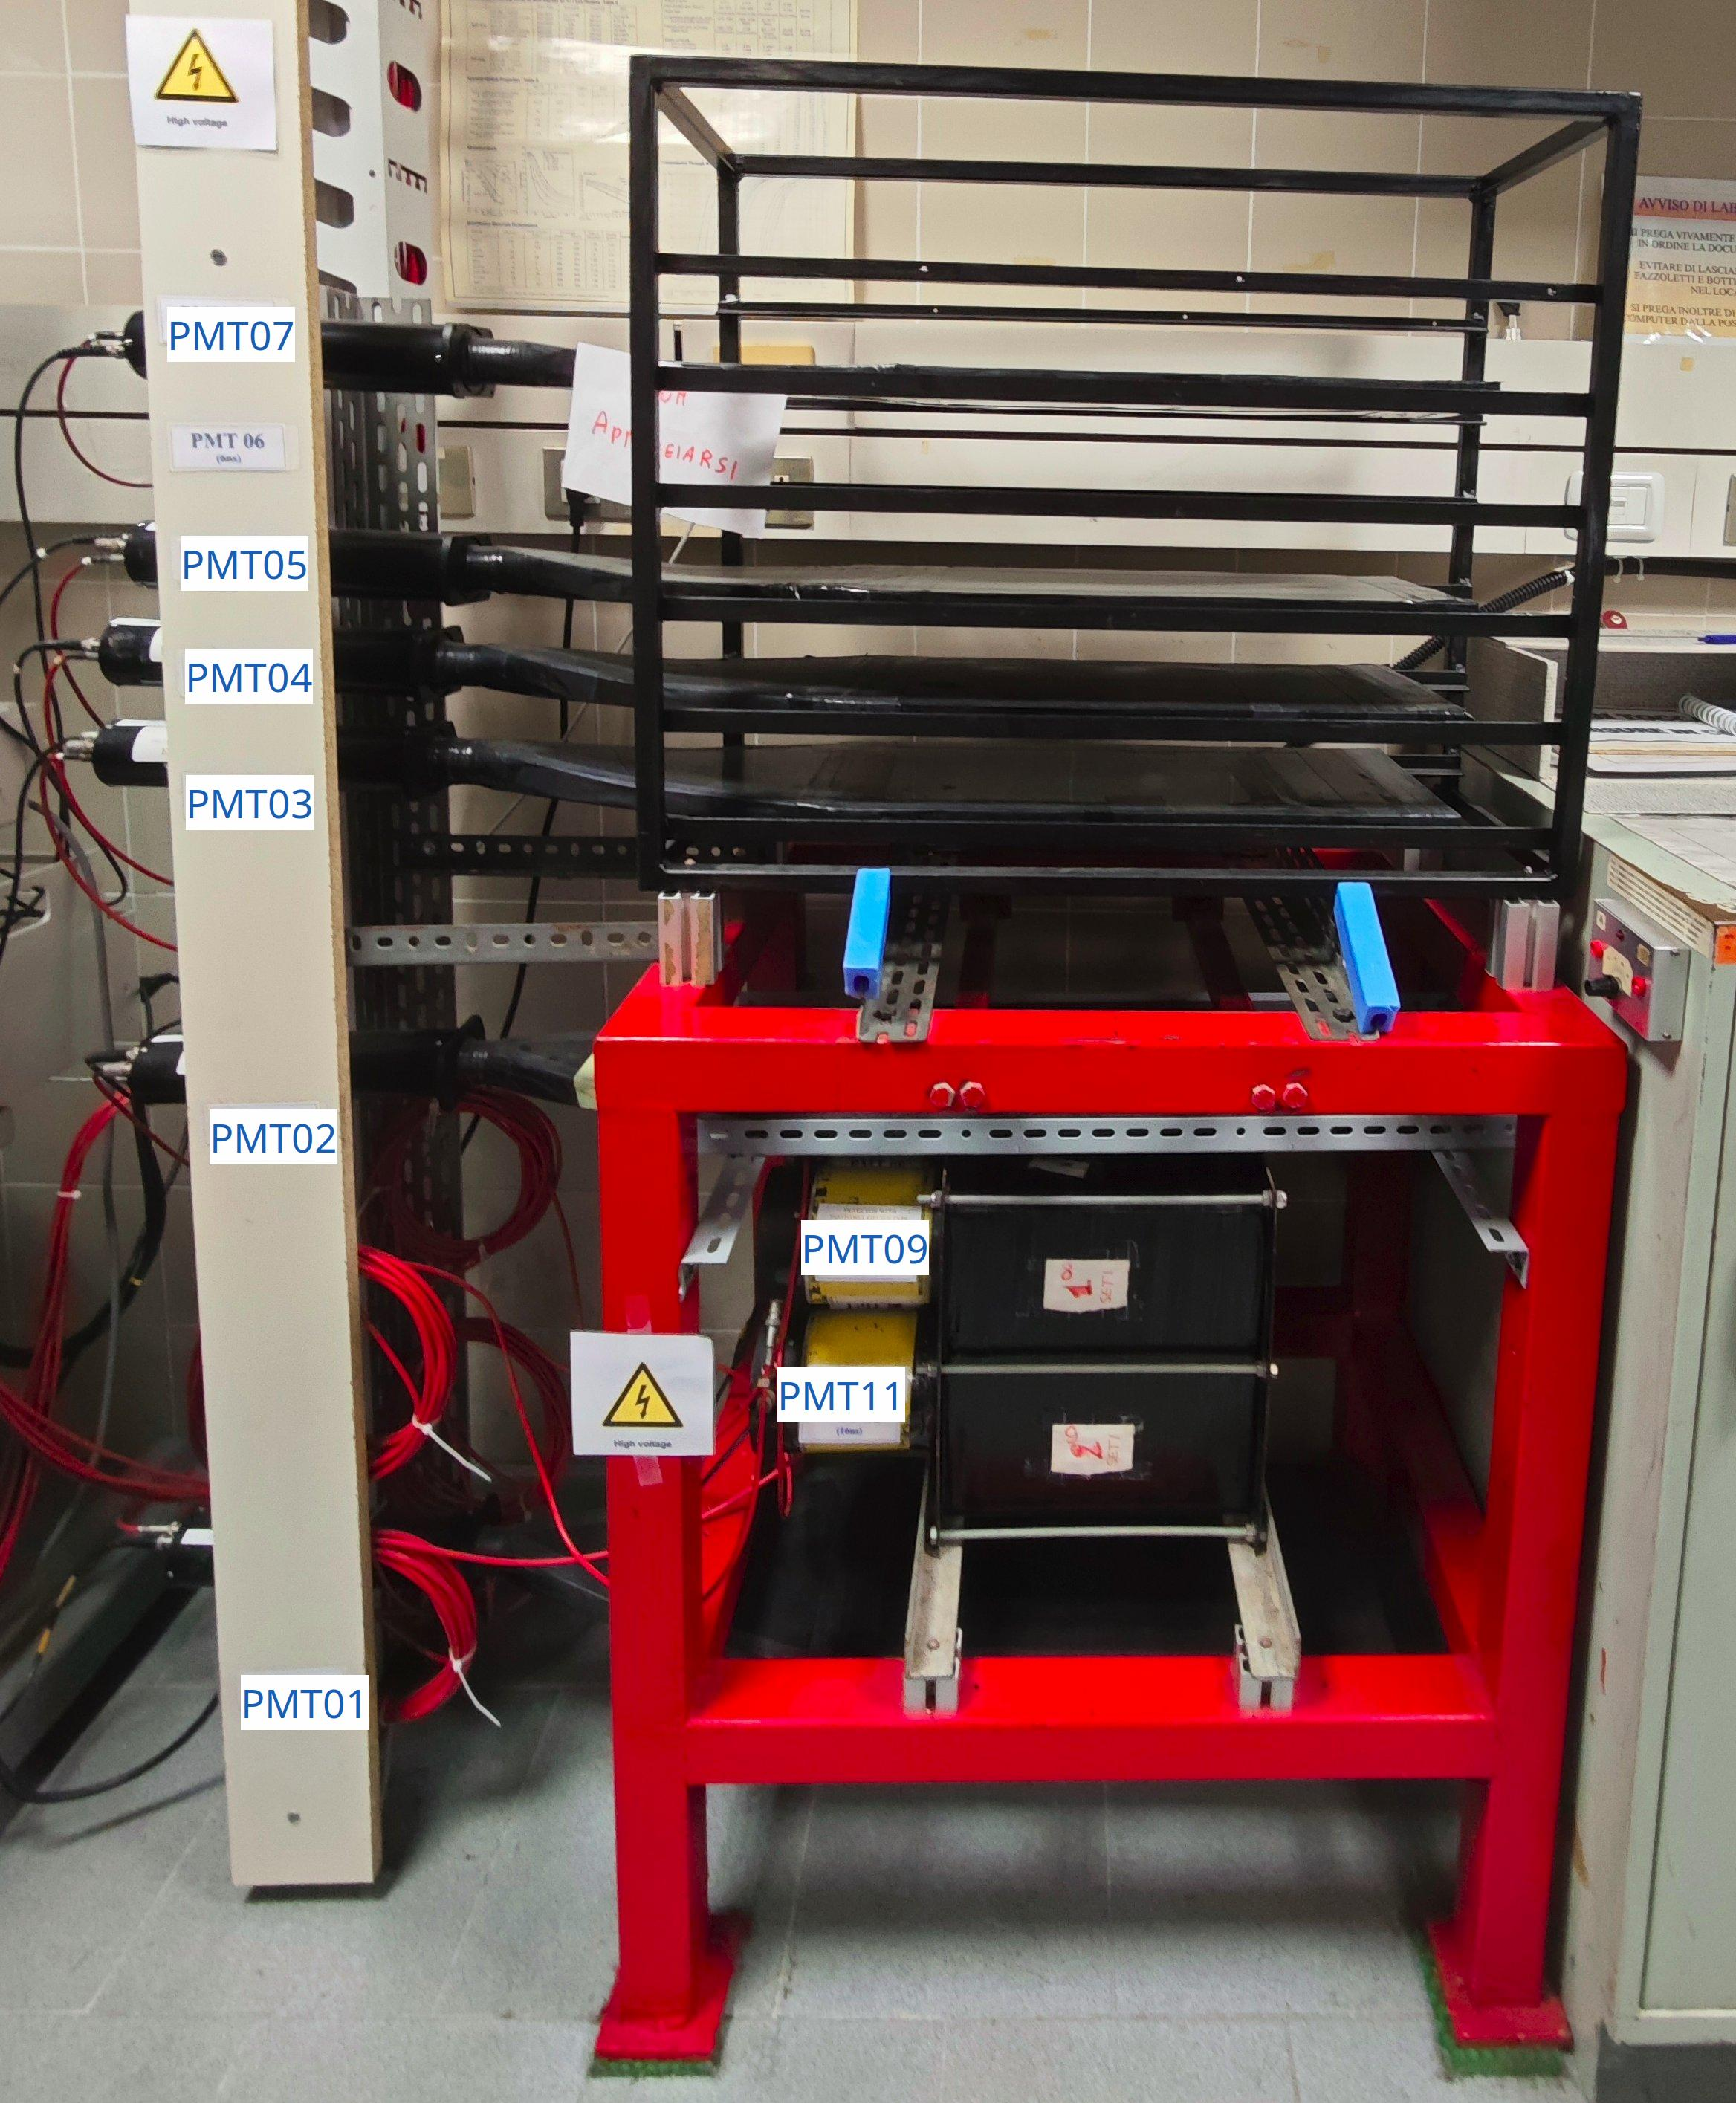
\includegraphics[width = 0.85\textwidth]{Immagini/apparato1.jpg}
        \caption{Scintillatori e PMT a disposizione}
        \label{fig:telescopio}
    \end{figure}
    \end{minipage}
    \hfill
    \begin{minipage}{0.48\linewidth}
    \begin{figure}[H]
    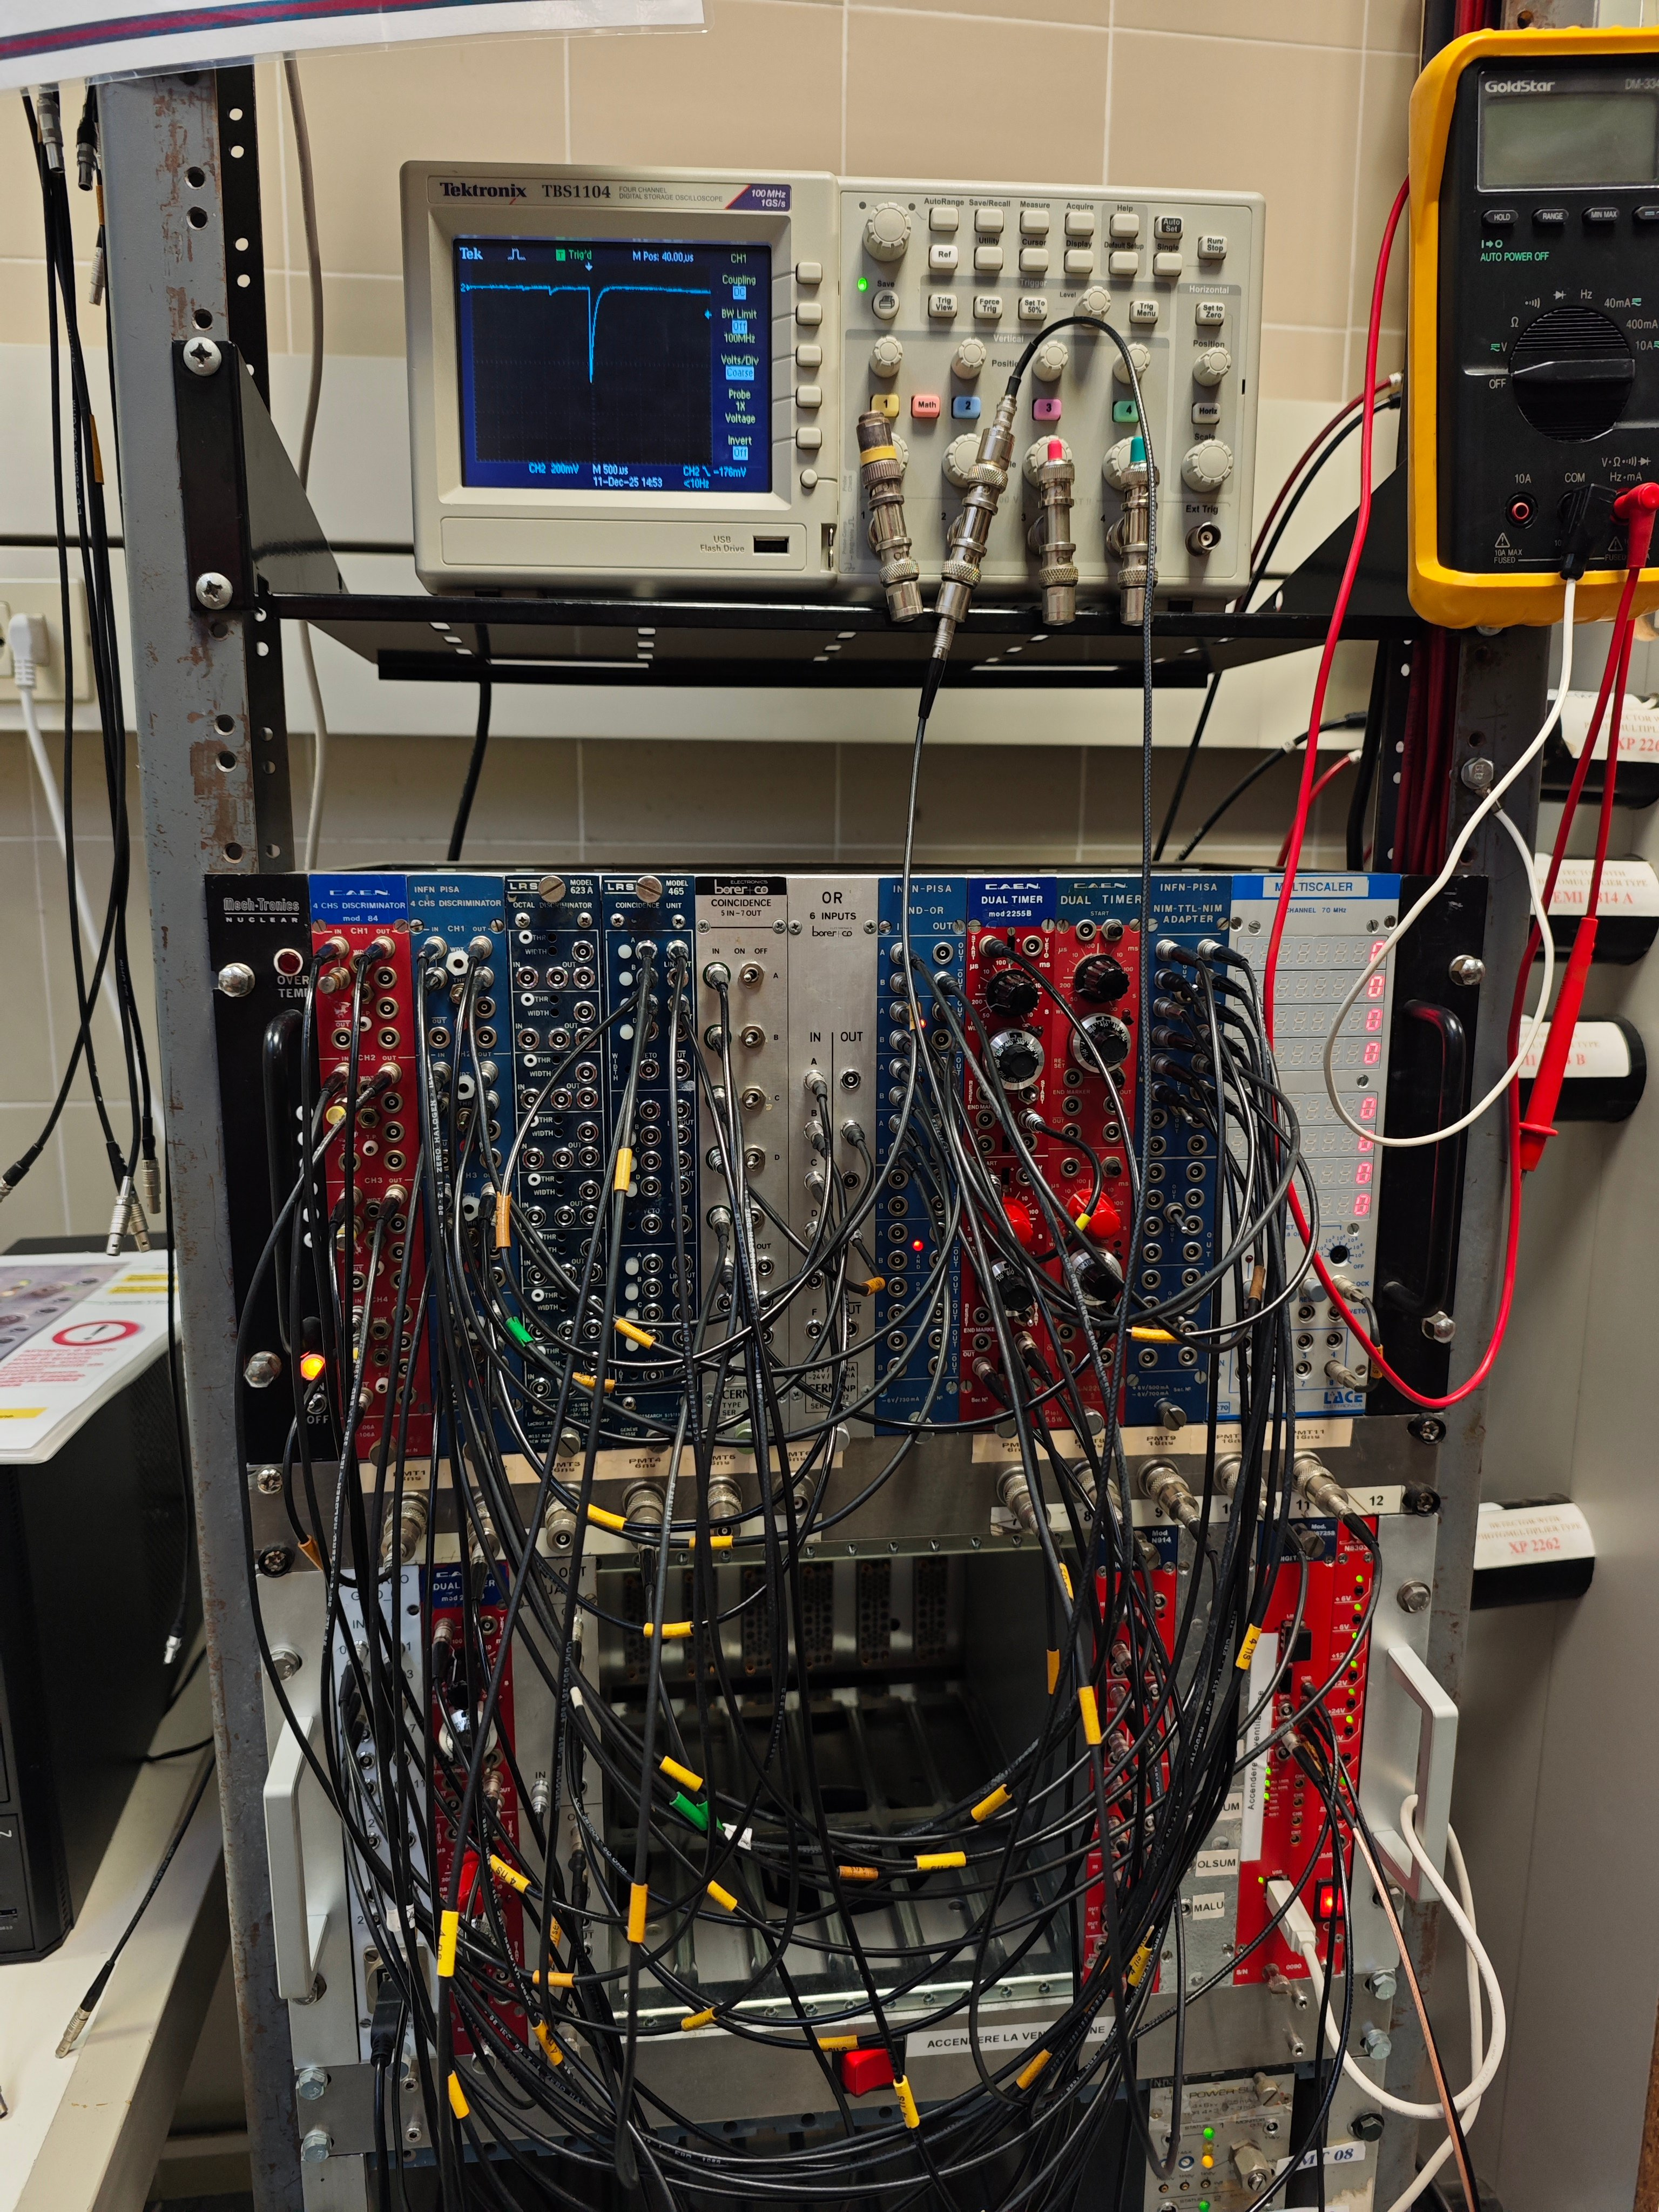
\includegraphics[width = 0.85\textwidth]{Immagini/moduli1.jpg}
    \caption{Rack con alcuni moduli utilizzati}
    \label{fig:rack}
    \end{figure}
    \end{minipage}



Gli strumenti e i moduli logici utilizzati nel corso dell'esperienza sono:
\begin{itemize}
\item Alimentatore alto voltaggio CAEN R1470ET
\item 6 lastre di scintillatore a disposizione per il telescopio ((49.8 $\pm$ 0.1 cm) $\times$ (27.5 $\pm$ 0.1 cm) $\times$ (2.3 $\pm$ 0.1 cm)), collegate ciascuna a un fotomoltiplicatore (PMT 1-2-3-4-); 
\item 1 blocco di scintillatore (bersaglio) dimensioni (30.0 $\pm$ 0.1 cm) $\times$ (31.0 $\pm$ 0.1 cm) $\times$ (31.0 $\pm$ 0.1), collegato a 4 PMT; 
\item una scheda di sviluppo con FPGA DE0-10 NANO;
\item 2 discriminatori (NIM CAEN N84 e NIM INFN);
\item 3 unità di coincidenza (NIM LRS 465, NIM CERN N6234, NIM);
\item 1 unità di OR (NIM CERN);
\item 2 unità di Dual Timer (NIM CAEN mod2255B e NIM CAEN N2255);
\item 1 unità di conversione NIM-TTL (NIM INFN);
\item 1 multiscaler (NIM INFN Multiscaler130);
\item 1 unità di Fan-Out (NIM CERN);
\item 1 integratore analogico (NIM CAEN N914);
\item 1 ADC (NIM CAEN N6725);
\item 1 oscilloscopio (Tektronix);
\item 2 computer, per regolare le alimentazioni e per le acquisizioni;
\item 1 multimetro digitale;
\item cavi coassiali di vario ritardo e terminazioni a 50 e 0 $\Omega$;
\item 1 metro a nastro;
\end{itemize}

\section{Punto di lavoro}\label{sec:Punto_lavoro}

\subsection{Telescopio} \label{subsec:telescopio}
\begin{flushleft}
Per il telescopio abbiamo selezionato le lastre collegate ai PMT07-04-02 visibili nell'immagine \ref{fig:telescopio} .\\
La prima attività svolta è stato scegliere il punto di lavoro dei vari PMT. Soglie e alimentazioni influenzano l'efficienza e di conseguenza il numero di eventi rivelati. Vogliamo che questa sia più alta possibile in modo da massimizzare la statistica a nostra disposizione. 

Dopo una fase di test in cui abbiamo osservato il rate in singola dei vari PMT, sono stati scelti il PMT07, il PMT04 e il PMT02. Come stima dell'efficienza di un PMT (ad esempio il PMT07) abbiamo usato il rapporto fra le coincidenze triple $(07\land04\land02)$ e le coincidenze doppie degli altri due (nell'esempio $(04\land02)$). 

Misuriamo i conteggi combinando i segnali discriminati tramite le unità di coincidenza, le cui uscite sono in seguito inviate al multiscaler, che conta per 100 s. La misura viene poi ripetuta variando la tensione di alimentazione.

Durante la procedura sono state misurate anche le singole dei due PMT usati per le coincidenze doppie, in quanto il loro rate in singola influenza il rate delle doppie false, ottenuto da:
\begin{equation}
    \label{fake}
    R_{fake} = R_1 R_2 (w_1 + w_2 - 2w)
\end{equation}

Dove $R_1$ e $R_2$ sono i rate in singola dei PMT di interesse, $w_1$ e $w_2$ sono le durate dei loro segnali discriminati (50 ns nel nostro caso). $w$ è la sovrapposizione temporale minima per avere una coincidenza, di 2 ns. Sceglieremo alimentazioni e soglie cercando di rendere il numero di doppie false trascurabile rispetto alle doppie misurate.


Tale procedura è ottimale per il PMT04, ma non per il PMT07 e PMT02, a causa della geometria del sistema. 
Per correggere tale effetto abbiamo usato un metodo Montecarlo per simulare il passaggio dei raggi cosmici attraverso il rivelatore, al fine di ricavare la probabilità che un raggio cosmico passi per un PMT dato il passaggio dagli altri due (accettanza). 
Dividendo il rapporto triple su doppie misurato con tale valore si ottiene una stima dell'efficienza . Stimiamo quindi l'errore sul rapporto triple su doppie con: 

\begin{equation}
    \label{error_eff}
    \sigma_{\varepsilon} = \sqrt{\frac{\varepsilon(1-\varepsilon)}{D}}
\end{equation}
\\
dove $D$ è il numero di doppie.


Riportiamo le misure fatte nelle tabelle sottostanti, le colonne sono voltaggio di alimentazione, efficienza, errore sull'efficienza e numero di doppie false:

    \begin{minipage}{0.3\linewidth}
    \begin{table}[H]
        \centering
        \resizebox{1\linewidth}{!}{    \begin{tabular}{cccc}
    \toprule
    $HV$[V] ($\pm$ 1V) & $\varepsilon$ [$\%$] & $\sigma_{\varepsilon}$[$\%$] & $D_{fake}$ \\
    \midrule
    1675 & 52 & $\pm$ 2 & 0.69 \\
    1700 & 70 & $\pm$ 2 & 0.65 \\
    1720 & 80 & $\pm$ 1 & 0.63 \\
    1730 & 81 & $\pm$ 1 & 0.59 \\
    1750 & 89 & $\pm$ 1 & 0.53 \\
    1775 & 80 & $\pm$ 1 & 0.54 \\
    1800 & 91 & $\pm$ 1 & 0.56 \\
    \bottomrule
    \end{tabular}}
        \caption{PMT02}
        \label{tab:PMT02}
    \end{table}    
    \end{minipage}
    \hfill
    \begin{minipage}{0.3\linewidth}
    \begin{table}[H]
        \centering
        \resizebox{1\linewidth}{!}{    \begin{tabular}{cccc}
    \toprule
    $HV$[V] ($\pm$ 1V)& $\varepsilon$ [$\%$] & $\sigma_{\varepsilon}$[$\%$] & $D_{fake}$ \\
    \midrule
    1675 & 87 & $\pm$ 2 & 0.077 \\
    1700 & 94 & $\pm$ 1 & 0.068 \\
    1720 & 94 & $\pm$ 1 & 0.074 \\
    1730 & 92 & $\pm$ 2 & 0.073 \\
    1750 & 93 & $\pm$ 1 & 0.078 \\
    1775 & 94 & $\pm$ 1 & 0.076 \\
    1800 & 92 & $\pm$ 1 & 0.076 \\
    \bottomrule
    \end{tabular}}
        \caption{PMT04}
        \label{tab:PMT04}
    \end{table}    
    \end{minipage}
    \hfill
    \begin{minipage}{0.3\linewidth}
    \begin{table}[H]
        \centering
        \resizebox{1\linewidth}{!}{    \begin{tabular}{cccc}
    \toprule
    $HV$[kV] ($\pm$ 1V)& $\varepsilon$ [$\%$] & $\sigma_{\varepsilon}$[$\%$] & $D_{fake}$ \\
    \midrule
    1.675 & 50 & $\pm$ 2 & 0.97 \\
    1.700 & 77 & $\pm$ 2 & 0.79 \\
    1.720 & 83 & $\pm$ 1 & 0.73 \\
    1.730 & 78 & $\pm$ 2 & 0.73 \\
    1.750 & 80 & $\pm$ 2 & 0.68 \\
    1.775 & 92 & $\pm$ 1 & 0.64 \\
    1.800 & 88 & $\pm$ 1 & 0.57 \\
    \bottomrule
    \end{tabular}}
        \caption{PMT07}
        \label{tab:PMT07}
    \end{table}
    \end{minipage}
    

\hfill

    \begin{minipage}{0.56\linewidth}
    \begin{figure}[H]
    \label{Eff_curv_telescope}
    \centering
    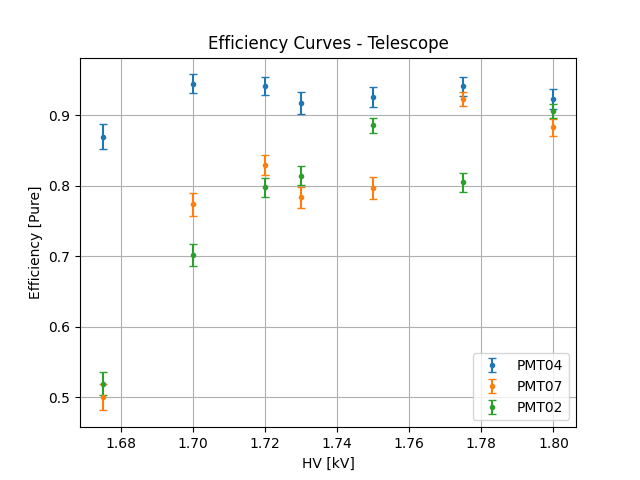
\includegraphics[width = 0.75\textwidth]{Grafici/Efficiency Curves - Telescope.png}
    \caption{Grafico delle curve di efficenza per i PMT02-04-07}
\end{figure}
    \end{minipage}
    \begin{minipage}{0.4\linewidth}
    \begin{table}[H]
        \centering
        \resizebox{1\linewidth}{!}{\begin{tabular}{cccc}
\toprule
Parametro & PMT02 & PMT04 & PMT07 \\
\midrule
$V_{supply}$ [V] & 1750 & 1700 & 1750 \\
$V_{thr}$ [mV] & -30 & -30 & -30 \\
$\varepsilon$ [$\%$] & 88 & 94 & 79 \\
\bottomrule
\end{tabular}}
        \caption{Punto di lavoro scelto per i PMT del telescopio}
        \label{tab:work_scope}
        \end{table}
    \end{minipage}
\vspace{0.5cm}\\
I parametri di lavoro scelti per i vari PMT del telescopio sono riportati in tabella \ref{tab:work_scope}

\end{flushleft}


\subsection{Bersaglio}\label{subsec:bersaglio}

\begin{flushleft}
Come riportato nella sezione \ref{subsec:telescopio}, dopo un fase di test preliminare siamo passati alla presa dati per la stima di efficienza dei PMT del blocco del bersaglio.
Per fare ciò è necessario ricostruire la curva di efficienza di tali PMT al variare della tensione di alimentazione. 
Al fine di creare una geometria favorevole alla misura, abbiamo usato diverse combinazioni di scintillatori in modo che il rivelatore del quale veniva misurata l'efficienza risultasse posizionato in mezzo agli altri due.
Riportiamo quindi le combinazioni usate per ciascun PMT del blocco:

\begin{itemize}

\item PMT08 : PMT02-PMT08-PMT10 
\item PMT09 : PMT02-PMT09-PMT01
\item PMT10 : PMT07-PMT08-PMT10
\item PMT11 : PMT09-PMT11-PMT01

\end{itemize}

Nel caso del PMT10 è stato necessario adottare un'altra metodologia in quanto la porzione di lastra ad esso vicino risulta essere fuori asse e non ampiamente sovrapposta con quella collegata al PMT01 (sotto) e non è sembrato quindi ragionevole usare la procedura della sezione \ref{subsec:telescopio}. In questo caso invece utilizziamo le lastre collegate ai PMT08 e PMT07. Questa geometria impone una verticalità sulla traiettoria dei raggi cosmici che attraversano i primi due piani di scintillatori in quanto molto ravvicinati. Desideriamo traiettorie più ortogonali possibili in quanto massimizzano la probabilità che dato il passaggio nelle due lastre soprastanti si abbia il passaggio anche nel bersaglio. Il calcolo effettuato è stato approfondito in appendice \ref{app:target_PMT10}.
Le misure di rate così come le stime di errore si sono svolte come descritto nella sezione \ref{subsec:telescopio}.
Riportiamo come nella sezione \ref{subsec:telescopio} il grafico realizzato per il rapporto triple su doppie (i dati sono riportati in appendice \ref{app:target}):
    \begin{minipage}{0.56\linewidth}
    \begin{figure}[H]
        \centering
        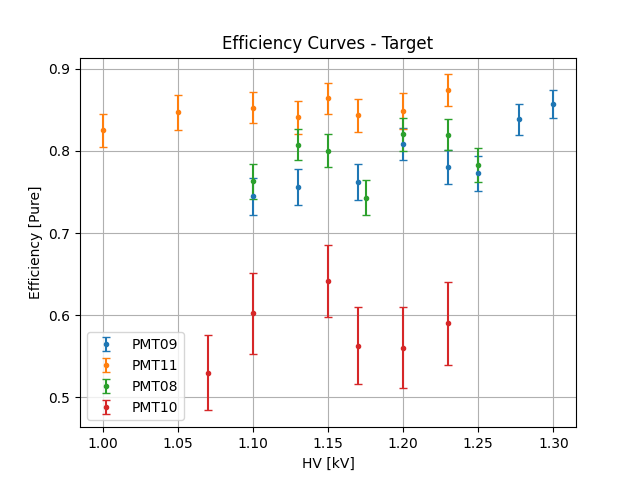
\includegraphics[width=1\linewidth]{Grafici/Efficiency Curves - Target.png}
        \caption{Curve di efficienza per i PMT di lettura del bersaglio}
    \label{fig:target}
    \end{figure}
    \end{minipage}
    \begin{minipage}{0.4\linewidth}
    \begin{table}[H]
        \centering
        \resizebox{1\linewidth}{!}{\input{Tabelle/work_target}}
        \caption{Punto di lavoro scelto per i PMT del blocco bersaglio}
        \label{tab:work_targ}              
        \end{table}
    \end{minipage}
\vspace{0.5cm}\\
Le condizioni di lavoro dei PMT del bersaglio sono quindi riportate nella tabella \ref{tab:work_targ}




\end{flushleft}
\newpage
\subsection{VETO}\label{subsec:veto}

\begin{flushleft}    

Infine abbiamo eseguito lo studio analogo per il PMT01(VETO). Abbiamo usato il rapporto triple su doppie della terna PMT07 - PMT09 $\vee$ PMT11 - PMT01. 

Il ragionamento per la scelta della terna delle lastre è lo stesso del caso precedente del PMT10, in quanto non è presente una lastra sottostante a quella del PMT01, dunque il metodo dei trigger ortogonali non ci è risultato ottimale per la misura.

\begin{table}[H]
    \begin{minipage}{0.5\linewidth}
        \centering
        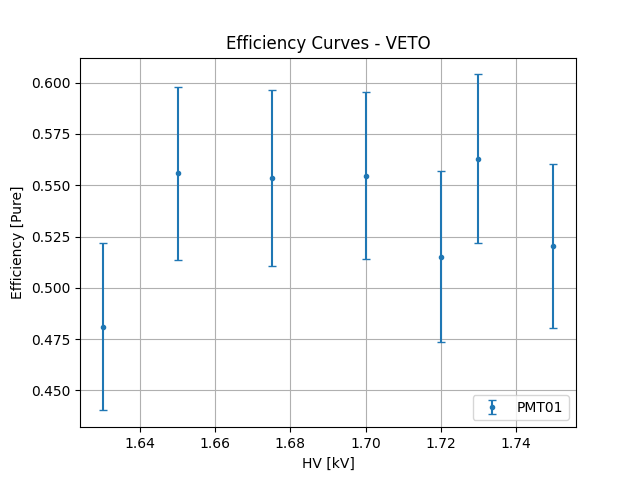
\includegraphics[width=0.91\linewidth]{Grafici/Efficiency Curves - VETO.png}
        \caption{Curva di efficienza per il PMT01(VETO)}
        \label{fig:veto_efficiency}
    \end{minipage}
    \begin{minipage}{0.5\linewidth}
        \centering
        \resizebox{0.7\linewidth}{!}{\begin{tabular}{cccc}
\toprule
HV [kV] & $\varepsilon [\%]$ & $\sigma_{\varepsilon} [\%]$ & $D_{fake}$ \\
\midrule
1.630 & 48 & $\pm$ 4 & 0.35 \\
1.650 & 56 & $\pm$ 4 & 0.35 \\
1.675 & 55 & $\pm$ 4 & 0.33 \\
1.700 & 55 & $\pm$ 4 & 0.34 \\
1.720 & 52 & $\pm$ 4 & 0.34 \\
1.730 & 56 & $\pm$ 4 & 0.33 \\
1.750 & 52 & $\pm$ 4 & 0.36 \\
\bottomrule
\end{tabular}}
        \caption{Dati utilizzati per la realizzazione del grafico \ref{fig:veto_efficiency}}
        \label{tab:work_targ}              
    \end{minipage}
\end{table}
In definitiva dopo aver analizzato il grafico \ref{fig:veto_efficiency} è stato scelto quindi come tensione di alimentazione $HV=1700$V.
\end{flushleft}
\subsection{Punto di lavoro e soglie}
Si riporta per completezza una tabella riassuntiva dei punti di lavoro di tutti i PMT utilizzati, le soglie dei discriminatori ai quali sono collegati e la loro efficienza a quella determinata tensione.
\begin{table}[H]
        \centering
        \resizebox{0.35\linewidth}{!}{\begin{tabular}{llll}
\hline
PMT & HV {[}V{]} & $\varepsilon$ {[}\%{]} & $V_{thr}${[}mV{]} \\ \hline
07  & 1750       & 79              & -30               \\
04  & 1700       & 94              & -30               \\
02  & 1750       & 88              & -30               \\
08  & 1260       & 78              & -40               \\
09  & 1320       & 85              & -40               \\
10  & 1260       & 58              & -40               \\
11  & 1260       & 87              & -40               \\
01  & 1700       & 55              & -30               \\ \hline
\end{tabular}}
        \caption{Condizioni di lavoro generali dell'apparato}
        \label{tab:work_general}     
\end{table}
\newpage

\section{Presa dati}\label{sec:presa_dati}

\subsection{Logica dei segnali}\label{subsec:logica_segnali}
\begin{flushleft}
Per la misura del tempo di decadimento abbiamo implementato una logica di START-STOP con VETO realizzata mediante opportune combinazioni dei segnali logici discriminati\footnote{Da qui in poi ci riferiremo ai segnali dei vari PMT solamente utilizzando il loro numero in riferimento al nostro apparato come riportato in sezione \ref{sec:apparato}} dei vari PMT e di segnali ausiliari generati con una logica secondaria.
Si riporta uno schema logico del circuito da noi realizzato:
\begin{figure}[H]
    \centering
    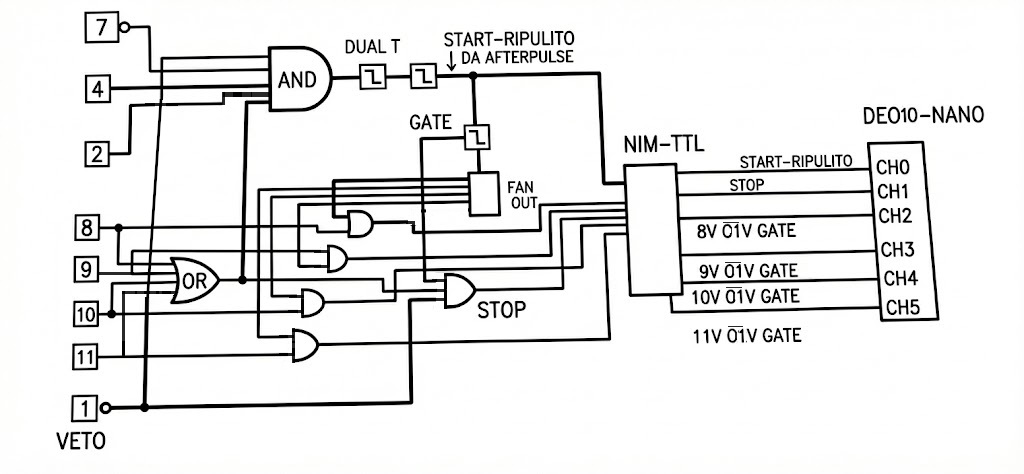
\includegraphics[width=0.7\linewidth]{Immagini/circuit.jpg}
    \caption{schema logico del setup sperimentale implementato.}
    \label{fig:logic_setup}
\end{figure}
Nel circuito di figura \ref{fig:logic_setup} possiamo quindi vedere:
\begin{itemize}
    \item \textbf{VETO: $\bm{\bar{(01)}}$}, segnale proveniente dal PMT01 collegato alla lastra scintillatrice più in basso, necessario per rivelare il passaggio di un raggio cosmico attraverso tutti i piani dell'apparato e di conseguenza scartare l'evento. Si utilizza  il segnale negato per necessità di logica in quanto siamo interessati a eventi di muoni che si fermano nel blocco del bersaglio.
    \item \textbf{START}: $\bm{(07\land04\land02)\land(08\lor09\lor10\lor11)\land (\bar{01})}$, La coincidenza tripla dei PMT del telescopio individua l'arrivo di un raggio cosmico, l'OR dei PMT del blocco ci dice che è passato per il blocco, mentre la coincidenza negata con il segnale di VETO rimuove eventi in cui il raggio cosmico attraverso l'apparato.
    \item \textbf{GATE}: Segnale generato con un dual timer che apre una finestra di 20$\mu \text{s}$, sul fronte di salita dello start. Necessario per filtrare a livello logico eventi indesiderati che non rappresentano decadimento del muone\footnote{La probabilità che accada dopo 20 $\mu s$ considerando il valore della vita media del muone nel carbonio riporatato nella sezione \ref{sec:intro} $P(t>20\mu \text{s})=\int_{20\mu s}^{+\infty}\exp{-t/ \tau_{\mu}} \text{ }dt = 4.77\cdot 10^{-5}\simeq 0.005 \%$}.
    \item \textbf{STOP: $\bm{(08\lor09\lor10\lor11) \land \text{GATE} \land (\bar{01}) }$}, Segnale di OR dei vari scintillatori del blocco del bersaglio in coincidenza con il GATE per filtrare eventi indesiderati, in coincidenza con il VETO per assicurarci che il segnale bersaglio non provenga da un cosmico che arriva in quella finestra di tempo \footnote{La probabilità che questo accada è esigua,in $\Delta t= 20\mu$s considerado il processo poissoniano con rate di $R =\Phi * A=15  s^{-1}$ dove approssimiamo il nostro rivelatore a un cubo di lato $l=30\text{cm}$ e utilizziamo il valore tipico di $\Phi =1 \text{cm}^{-2} \text{min}^{-1} $, otteniamo una probabilità $P(N\geq 2)\simeq(R\Delta t)^2\simeq 4.5\cdot10^{-8}$ }
    \item $\textbf{START\_RIPULITO}$: Il segnale di START una volta generato viene "ripulito" usandolo come input di un dual timer che apre una prima finestra di 150ns (allo scopo di eliminare treni di impulsi sullo START) questa finestra viene poi ridotta nuovamente a un segnale di 50ns per comodità utilizzando il secondo modulo del dual timer.
       
\end{itemize}

Si è inoltre dovuto regolare opportunamente le durate dei vari segnali discriminati in maniera da garantire la sovrapposizione necessaria per far si che le unità di coincidenzaregistrino la sovrapposizione per generare un segnale. Allo stesso modo è necessario non estendere eccessivamente la lunghezza temporale dei segnali in quanto come si nota in \ref{fake} questa è direttamente proporzionale al rate delle coincidenze false. Di conseguenza è sembrato ragionevole per tutti i segnali dei PMT scegliere una durata di 50 ns, ad eccezione per il PMT01(VETO).
Per tale segnale è stata impostata la durata di 100 ns e anticipato di 4 ns rispetto agli altri con opportune combinazioni di cavi. 
La ragione di questa scelta è che il VETO deve impedire che si generi un segnale di START non appena è determinato che l'evento non corrisponde a un muone fermatosi nel blocco. Quindi vogliamo sia in anticipo e più duraturo degli altri segnali con il quale è in coincidenza, in modo che la coincidenza risulti falsa per tutta la durata.
Da notare che per la logica scelta a ogni START corrisponde uno STOP molto ravvicinato. Si è deciso di non filtrarli via hardware, bensì di tenerne conto in sede di analisi dati in maniera da mantenere la logica semplice e avere più informazioni in sede di analisi dati.

\end{flushleft}

\subsection{Acquisizione dati}\label{subsec:logica_prog}

Tramite un'opportuna scelta dei segnali collegati alla scheda di sviluppo DEO10-nano sono state effettuate le prese dati necessarie alla determinazione della vita media del muone. Alla scheda sono stati quindi collegati i seguenti segnali: lo START\_RIPULITO(CH0), lo STOP(CH1) e 4 segnali aggiuntivi ottenuti dalla coincidenza del GATE con ciascuno dei PMT del blocco in OR con il negato del VETO(CH2-3-4-5).
I segnali di ogni singolo PMT del bersaglio sono stati importanti in fase di analisi dati in quanto hanno permesso di ricostruire in maniera ottimale gli intervalli di tempo e fornito informazioni sul comportamento dei singoli PMT del bersaglio.\\
L'algoritmo implementato per la ricostruzione degli intervalli di tempo ha una logica di tipo \textit{greedy pairing}\footnote{Algoritmo che una volta individuato uno Start scorre gli Stop che seguono temporalmente e lo accoppiano al primo segnale di stop che rispetta una determinata condizione} in breve:
\begin{itemize}
\item Individua uno START;
\item Controlla ci sia uno STOP, oppure uno STOP con segnale in uno dei PMT, oppure STOP con segnale in due PMT sovrapposti contemporaneamente;
\item Ripete il controllo cercando i casi precedenti o alternativamente segnale in uno dei PMT;
\item Fa la differenza fra lo START trovato all'inizio e il primo STOP utile.
\end{itemize}
Per una descrizione più approfondita si rimanda all'appendice \ref{app:logica_prog_1}
\section{Analisi dati}\label{sec:analisi_dati}

\subsection{Modellizzazione}\label{subsec:modelliz}

\begin{flushleft}
    
Terminata la presa dati abbiamo realizzato l'istogramma dei tempi di decadimento $dt$, per fare questo è stato necessario realizzare un codice \texttt{ROOT} per implementare la logica necessaria ad interpretare i dati e ricostruire gli intervalli di tempo.\\
L’istogramma dei tempi di decadimento $d t$ realizzato contiene conteggi interi $n_i$ per ciascun bin temporale $i$, consideriamo quindi la distribuzione di tipo poissoniano. Nel fit assumiamo quindi che, a parametri $\theta=(N_0,\tau,B)$ fissati, i conteggi dei bin siano variabili aleatorie indipendenti distribuite come
\begin{equation}
n_i \sim \mathrm{Poisson}\!\left(\mu_i(\theta)\right),
\end{equation}
dove $\mu_i(\theta)$ è il valore atteso nel bin $i$. La dipendenza temporale del valore atteso è modellata da un esponenziale più una costante di fondo,
\begin{equation}
\label{fit_func}
f(t;\theta)=N_0 e^{-t/\tau}+B,
\end{equation}
l'equazione \ref{fit_func} viene quindi implementata come funzione parametrica di fit. È stato in seguito realizzato un fit in \texttt{ROOT} per stimare il valore dei parametri $\theta$, per fare ciò abbiamo utilizzato le opzioni \texttt{LIR}, l'opzione \texttt{L} ci permette di fare un fit di massima likelihood.\\
Assumendo indipendenza tra bin, la likelihood binned Poisson è definita come:
\begin{equation}
\label{eq:likelihood}
\mathcal{L}(\theta)=\prod_i \frac{\mu_i(\theta)^{n_i}e^{-\mu_i(\theta)}}{n_i!}.
\end{equation}
da cui ricaviamo lo stimatore $\hat{\theta}$:
\begin{equation}
\label{eq:max_like}
\hat{\theta}=\arg\max_{\theta}\,\mathcal{L}(\theta)
\;\;\Leftrightarrow\;\;
\hat{\theta}=\arg\min_{\theta}\left[-\ln\mathcal{L}(\theta)\right],
\end{equation}
In pratica si minimizza la quantità $-\ln\mathcal{L}$ detta \textit{log-likelihood}.\\
L’opzione \texttt{I} impone l’uso dell’integrale della funzione nel bin\footnote{Utile sopratutto nella parte iniziale dell'esponenziale dove la funzione può variare molto dentro il bin stesso} quindi per un bin con estremi $(t_i^{-},t_i^{+})$ si ha
\begin{equation}
\label{eq:val_medio}
\mu_i(\theta)=\int_{t_i^{-}}^{t_i^{+}} f(t;\theta)\,dt
= N_0\,\tau\left(e^{-t_i^{-}/\tau}-e^{-t_i^{+}/\tau}\right) + B\,\Delta t_i,
\qquad \Delta t_i=t_i^{+}-t_i^{-}.
\end{equation}
Il fit viene quindi ristretto all’intervallo $t\in[t_{\min},t_{\max}]$ mediante l'opzione \texttt{R}  scelto per evitare problemi a piccoli tempi e in coda (vedi sezione \ref{subsec:sys_err}). \\

Nel caso del fit che abbiamo realizzato il $\chi^2$ non può essere indice della bontà del nostro fit in quanto non viene minimizzato nel processo di fit stesso.\\
Per avere una valutazione della bontà del fit realizzato quindi si introduce una quantità chiamata devianza definita come:

\begin{equation}
\label{eq:deviance}
D = -2\ln\!\left(\frac{\mathcal{L}(\hat{\theta})}{\mathcal{L}_\mathrm{sat}}\right)
=2\sum_i \left[n_i\ln\!\left(\frac{n_i}{\mu_i(\hat{\theta})}\right)-(n_i-\mu_i(\hat{\theta}))\right],
\end{equation}

con la convenzione $n_i\ln(n_i/\mu_i)=0$ per $n_i=0$. In condizioni asintotiche $D$ è approssimativamente distribuita come $\chi^2$ con $\nu\simeq N_{\mathrm{bin}}-N_{\mathrm{par}}$ gradi di libertà, consentendo un test globale di goodness-of-fit. Per un'analisi completa sono stati anche calcolati i residui di devianza bin-per-bin definiti come:
\begin{equation}
\label{eq:residual}
r_{D,i}=\mathrm{sign}\!\left(n_i-\mu_i(\hat{\theta})\right)
\sqrt{2\left[n_i\ln\!\left(\frac{n_i}{\mu_i(\hat{\theta})}\right)-(n_i-\mu_i(\hat{\theta}))\right]},
\qquad \sum_i r_{D,i}^2 = D,
\end{equation}
questi che verranno riportati nei grafici realizzati nelle sezioni successive permettono di identificare eventuali effetti sistematici non compatibili con fluttuazioni poissoniane attorno al modello.\\
In particolare in particolari condizioni (conteggi non troppo piccoli, bin indipendenti, modello correttamente specificato) i residui $r_{D,i}$ risultano approssimativamente distribuiti come una normale standard:
\begin{equation}
\label{eq:res:dist}
r_{D,i}\ \approx\ \mathcal{N}(0,1),
\end{equation}

\subsection{Fit vita media}
\label{subsec:fit_vita_media}
Controllando che le condizioni di lavoro dell'apparato rimanessero invariate, abbiamo effettuato diverse prese dati per massimizzare la statistica a nostra disposizione e migliorare la misura della vita media.
Riportiamo quindi una tabella riassuntiva delle varie prese dati effettuate.
\vspace{1cm}
\begin{table}[H]
        \centering
        \resizebox{0.5\linewidth}{!}{\begin{tabular}{llll}
\hline
\#presa dati & data inizio & data fine  & durata \\ \hline
1            & 28/11/2025  & 02/12/2025 & 100h   \\
2            & 02/12/2025  & 03/12/2025 & 20h    \\
3            & 04/12/2025  & 09/12/2025 & 96h    \\ \hline
\end{tabular}
}
        \caption{Elenco delle varie prese dati con datazione e durata}
        \label{tab:takes}
\end{table}
\newpage
Combinando i dataset di tabella \ref{tab:takes} è stato quindi realizzato l'istogramma dei dt di decadimento ricostruiti come descritto in \ref{subsec:logica_prog} e realizzato il fit secondo le procedure della sezione \ref{subsec:modelliz}.\\
\begin{figure}[H]
    \centering
    \begin{minipage}{0.48\linewidth}
        \centering
        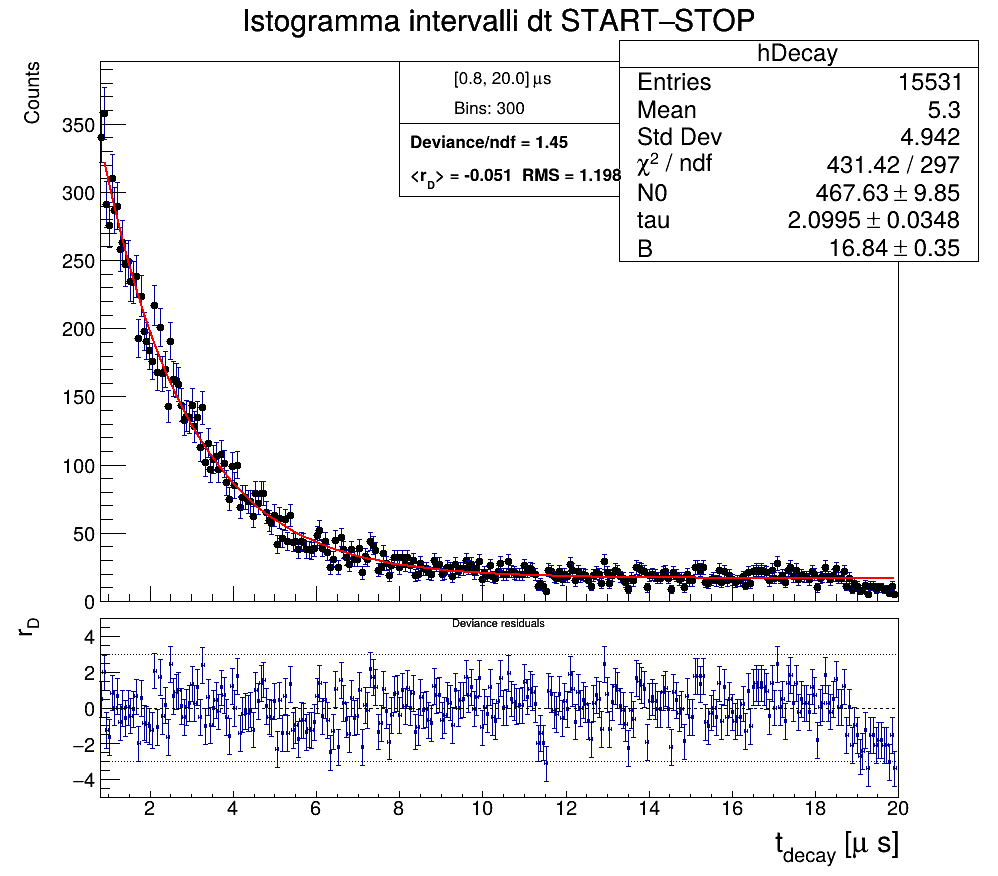
\includegraphics[width=\linewidth]{Grafici_fit_finale/mu_decay_fit_0.800_20.000_300_bins_withdevres.png}
        \caption{Risultati del fit con residui}
        \label{fig:fit}
    \end{minipage}
    \hfill
    \begin{minipage}{0.48\linewidth}
        \centering
        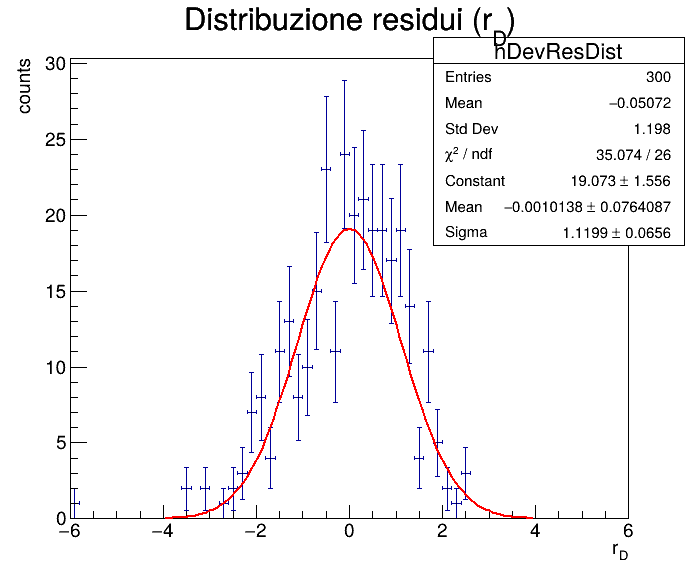
\includegraphics[width=\linewidth]{Grafici_fit_finale/devres_distribution_0.800_20.000_300_bins.png}
        \caption{Distribuzione dei residui}
        \label{fig:residui}
    \end{minipage}
\end{figure}
In questo caso è stato scelto di realizzare il fit degli intervalli $dt \in [0.8,20] \mu \text{s}$, nelle sezione \ref{subsec:sys_err} verrà approfondito il motivo di questa scelta, per ora ci limitiamo a fornire i risultati ottenuti.\\
Il fit restituisce un valore per vita media : $\bm{\tau = 2.099 \pm 0.035\mu}\textbf{s}$ e per gli altri parametri restituisce i valori $\bm{N_0=467 \pm 10 \textbf{ counts}}$ e $\bm{B= 16.8 \pm 0.3 \textbf{ counts}}$.\\
Come anticipato nella sezione \ref{subsec:modelliz} per completezza e per osservare eventuali problematiche nella presa dati o nelle procedure di fit (effetti sistematici) è stato realizzato anche un subplot dei residui visibile in figura \ref{fig:fit},questo non evidenzia criticità o andamenti particolari se non una tendenza negativa dei valori dei residui data da una sottopopolazione dei bin agli estremi dell'intervallo temporale di fit attorno a $t_{max}$.\\
Per completare ulteriormente l'analisi è stato realizzato anche un istogramma della distribuzione dei residui di devianza che come anticipato nella sezione \ref{subsec:modelliz} sotto determinate ipotesi dovrebbe tendere a una normale standard.\\
Pertanto ci si aspetta: per il grafico \ref{fig:residui} una distribuzione simmetrica attorno a zero; una media campionaria compatibile con zero e RMS$\simeq1$, nel grafico vengono poi riportate le seguenti grandezze:
\begin{equation}
<r_D>=\frac{1}{N}\sum_{i=1}^{N} r_{D,i},
\qquad
\mathrm{RMS}(r_D)=\sqrt{\frac{1}{N}\sum_{i=1}^{N} r_{D,i}^2}
=\sqrt{\frac{D}{N}},
\end{equation}
dove $N$ è il numero di bin inclusi nel fit. 
Valori RMS significativamente maggiore di 1 suggeriscono fluttuazioni più ampie di quelle poissoniane attese e un RMS minore di 1 può indicare correlazioni overfitting.\\
Nel nostro caso, la distribuzione dei residui di devianza (Fig.~\ref{fig:residui}) risulta ben descritta da una Gaussiana centrata in prossimità di zero: la media campionaria è $<r_D>\simeq -0.035$ e l’RMS $\simeq 1.05$, mentre un fit gaussiano fornisce $\mu_G \simeq (-0.054\pm 0.064)$ e $\sigma_G \simeq (1.02\pm 0.05)$, compatibili entro incertezze con le attese $\mu_G=0$ e $\sigma_G=1$.\\
Ciò supporta l’ipotesi che, nell’intervallo $[t_{\min},t_{\max}]$ adottato e con il modello esponenziale più fondo costante, le discrepanze osservate siano coerenti con fluttuazioni statistiche poissoniane.
Infine è stato calcolato il rapporto $D/ndof$ in condizioni asintotiche come descritto in sezione \ref{subsec:modelliz} la devianza è distribuita come un $\chi^2$, calcolando il rapporto quindi è possibile avere un ulteriore conferma della bontà del fit , il valore atteso per questo rapporto è $\hat{D/ndof}\simeq 1$, nel grafico \ref{fig:fit} otteniamo il risultato $D/ndof=1.45$ che non suggerisce particolari problemi.


\end{flushleft}

\subsection{Errori sistematici}\label{subsec:sys_err}
\begin{flushleft}


Al fine di comprendere il comportamento del fit realizzato abbiamo studiato la dipendenza della misura di vita media da vari parametri che rientrano nelle impostazioni di fit, scrivendo un codice in \texttt{ROOT} che realizzasse una scansione con varie combinazioni di:
\begin{itemize}
\item numero di bin $n_{bin}$: allo scopo di osservare se la densità di questi modifichi sensibilmente la misura ottenuta di vita media;
\item estremo inferiore del taglio temporale ($t_{min}$): Per studiare l'effetto del taglio iniziale dei dati, fondamentale per l'ottimizzazione della stima di vita media.
\item estremo superiore del taglio temporale ($t_{max}$): per studiare l'effetto del taglio sulle zone estreme dei tempi che potrebbero essere affette da effetti di bordo e tagli; 
\end{itemize}
Riportiamo quindi i grafici realizzati e le tabelle con le varie combinazioni di $n_{bin}$, $t_{min}$e $t_{max}$ esplorate:

\begin{table}[h]
\centering
\label{tab:combination}
\resizebox{0.25\linewidth}{!}{\begin{tabular}{lll}
\hline
$n_{bin}$ & $t_{min}$ $ [\mu \text{s}]$ & $t_{max}$ $[\mu \text{s}]$ \\ \hline
150       & 0.4                    & 10                    \\
200       & 0.6                    & 12                    \\
250       & 0.8                    & 15                    \\
300       & 1.0                    & 17                    \\
400       & 1.2                    & 18                    \\
500       & 1.4                    & 19                    \\
100       & 1.6                    & 20                    \\ \hline
\end{tabular}
}
\caption{Tabella dei valori dei parametri utilizzati per i test effettuati}
\end{table}

\begin{figure}[H]
    \centering
    \begin{minipage}{0.48\linewidth}
    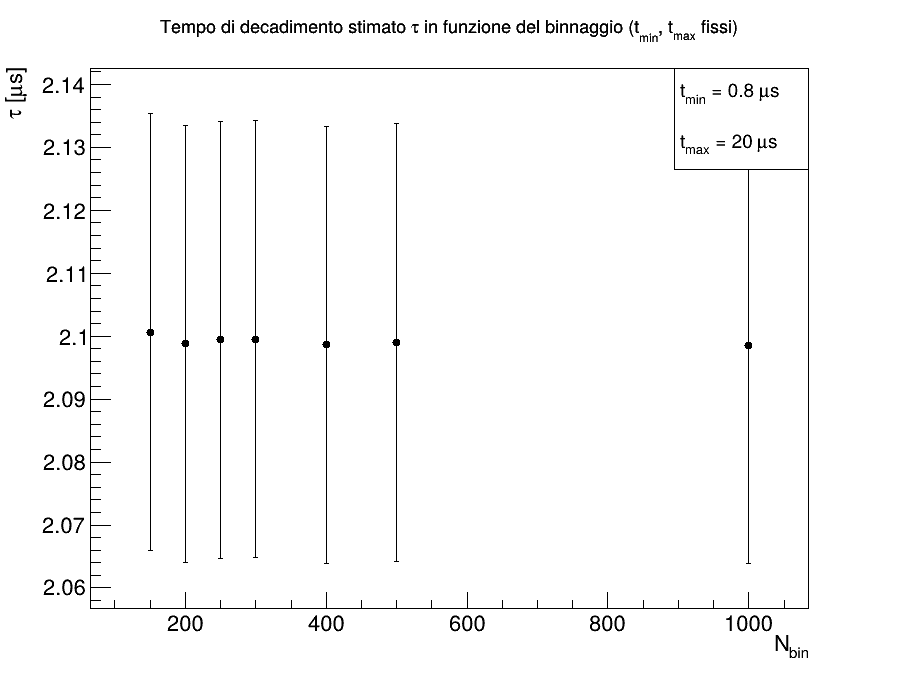
\includegraphics[width=0.8\linewidth]{Grafici_fit_finale/FIFO_combined_tau_vs_nbins_fixed.png}
    \caption{$\tau$ in funzione di $n_{bin}$, mantenendo gli altri parametri fissi}
    \label{fig:tau_bin}
    \end{minipage}
    \hfill
    \begin{minipage}{0.48\linewidth}
        \centering
        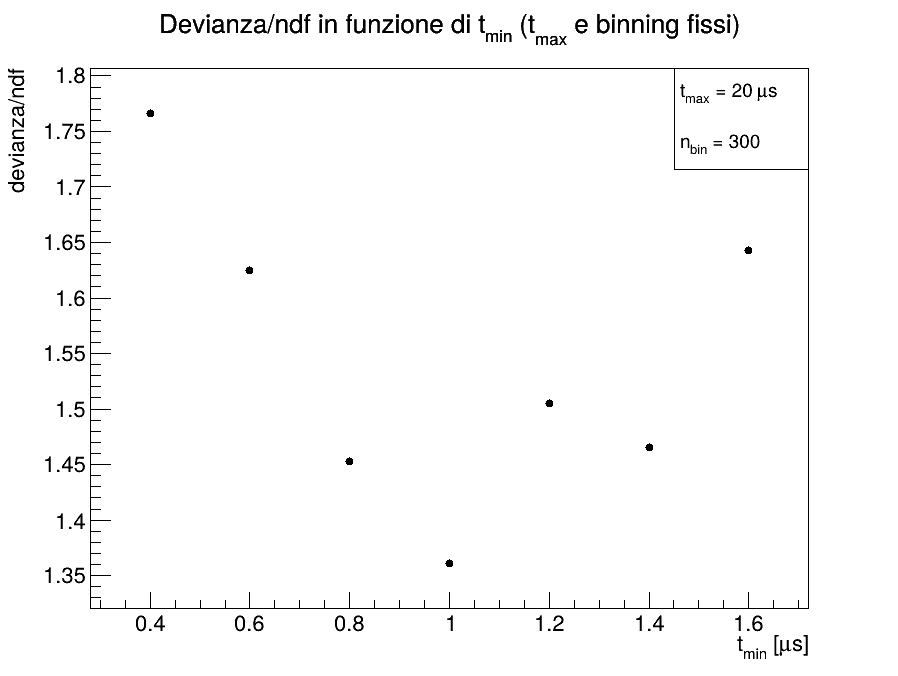
\includegraphics[width=0.8\linewidth]{Grafici_fit_finale/FIFO_combined_devOverNdf_vs_tmin_fixed.png}
        \caption{Rapporto devianza/ndof in funzione del $t_{min}$, mantenendo gli altri parametri fissi}
        \label{fig:deviance_ndof}
    \end{minipage}
\end{figure}
\hfill
\begin{figure}[H]
    \centering
    \begin{minipage}{0.48\linewidth}
        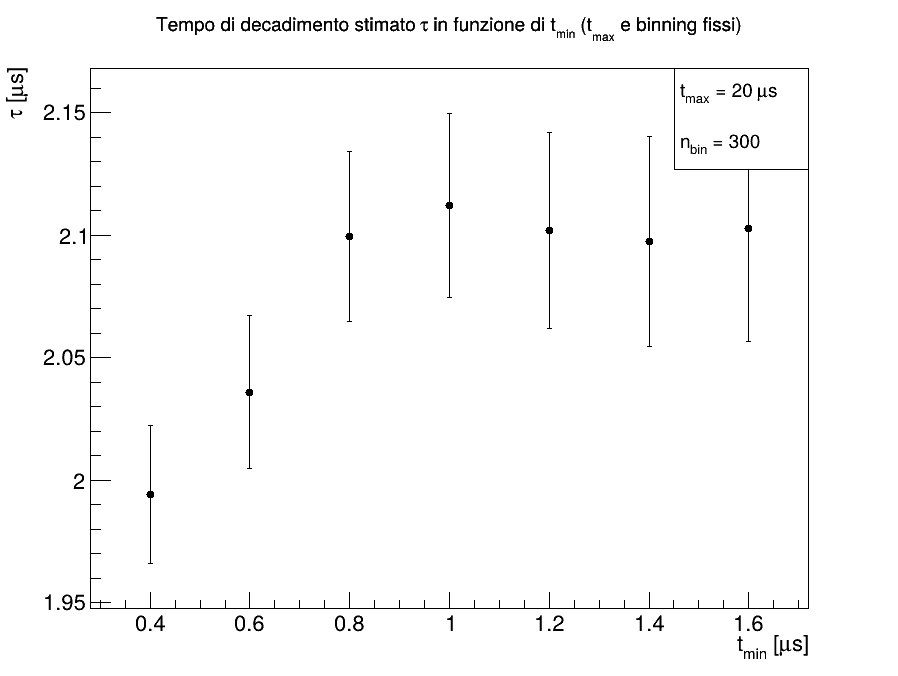
\includegraphics[width=0.8\linewidth]{Grafici_fit_finale/FIFO_combined_tau_vs_tmin_fixed.png}
        \caption{$\tau$ in funzione del $t_{min}$, mantenendo gli altri parametri fissi}
        \label{fig:tau_tmin}
    \end{minipage}
    \hfill
    \begin{minipage}{0.48\linewidth}
        \centering
        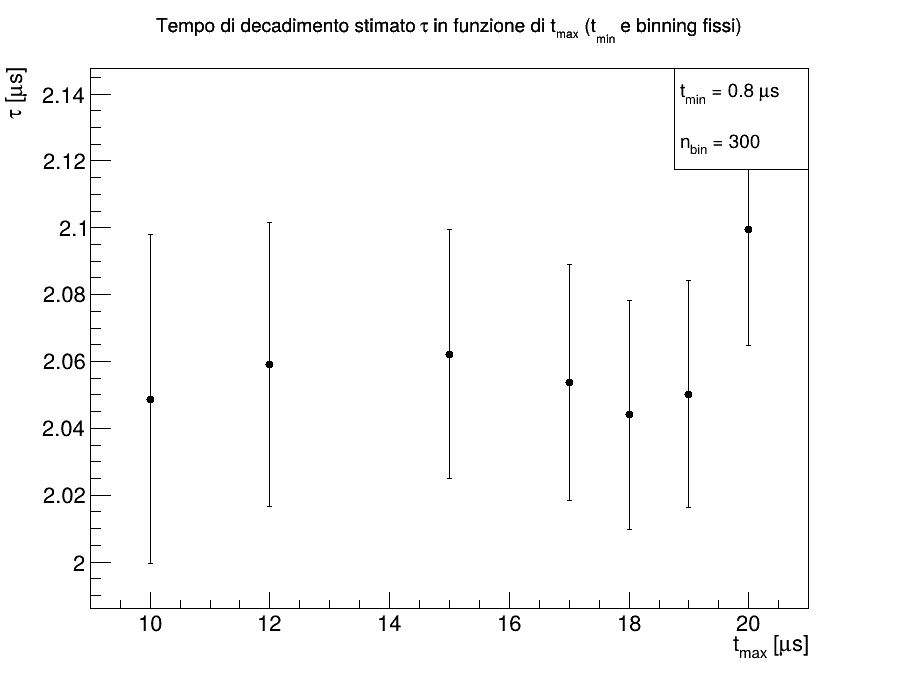
\includegraphics[width=0.8\linewidth]{Grafici_fit_finale/FIFO_combined_tau_vs_tmax_fixed.png}
        \caption{$\tau$ in funzione del $t_{max}$, mantenendo gli altri parametri fissi}
        \label{fig:tau_tmax}
    \end{minipage}
\end{figure}


Osservando il grafico \ref{fig:tau_bin}, osserviamo un andamento costante $\tau$ in funzione di $n_{bin}$ che evidenzia come a parametri fissati ($t_{min}$ e $t_{max}$) la misura di vita media ottenuta dal fit non dipenda dal binnaggio in prima analisi.\\
Osservando l'andamento di $\tau$ in funzione di $t_{min}$invece notiamo una dipendenza iniziale dal valore di questo parametro (variazione del 5\% da $0.4\mu$s a $0.8\mu$s), per poi raggiungere un plateau (zona da 0.8$\mu$ s in poi).\\
Combinando tutti i dataset a nostra disposizione e ricostruendo i gli intervalli di tempo osserviamo fin da subito che la maggior parte degli eventi da noi acquisiti consistono in falsi STOP dovuti sia alla logica in sé che fa corrispondere uno STOP ritardato in media di qualche decina di nanosecondi a seguito di uno START, sia a fenomeni di afterpulse e rumore di fondo, questo contamina il nostro dataset con una quantità di $dt$ falsi che senza adeguate attenzioni non permetterebbero l'analisi dati.\\
Si può notare infatti che nei primi 0.4 $\mu \text{s}$ sono stati ricostruiti $n_{dt\in[0,0.4]}= 87484 \text{ eventi} $, su un totale di $n_{tot}= 105723$ con un rapporto $R=83\%$, senza filtrare questi eventi non è possibile analizzare i dati a nostra disposizione.\\ 
Alla luce di questo, è stato deciso di adottare come estremo inferiore del nostro intervallo di tempo per il fit finale $t_{min}=0.8\mu$s, punto in cui si inizia ad osservare appunto il plateau.\\
Passando al grafico \ref{fig:tau_tmax} notiamo come non si abbia dipendenza particolare del valore di $\tau$ in funzione di $t_{max}$ fino ad arrivare al valore limite di 20$\mu$ s dove già durante l'analisi dell'andamento dei residui nella sezione \ref{subsec:fit_vita_media} nella figura \ref{fig:fit} aveva evidenziato criticità probabilmente dovute a effetti di bordo e di digitalizzazione.\\
Per questo è stato deciso di fissare $t_{max}=18 \mu $s nella realizzazione del fit finale.\\
il grafico \ref{fig:deviance_ndof} non mostra andamenti particolari di $D/ndof$ al variare di $t{min}$ è possibile che sia presente una dipendenza ma non è evidenziata da tale studio.\\
\end{flushleft}

\subsection{Fit finale}
\label{subsec:fit_final}
\begin{flushleft}
Al netto di tutte le considerazioni nella sezione \ref{subsec:sys_err} abbiamo deciso di ripetere le operazioni di fit per i parametri che sono sembrati ottimali, la procedura rimane invariata rispetto alla sezione \ref{subsec:fit_vita_media}
Si utilizza quindi la combinazione $\bm{t_{min}=0.8 \mu s}$, $\bm{t_{max}=18 \mu s}$ e $\bm{n_{bin}=300}$, si riportano quindi in seguito i grafici realizzati e i risultati ottenuti:
\begin{figure}[H]
    \centering
    \begin{minipage}{0.48\linewidth}
        \centering
        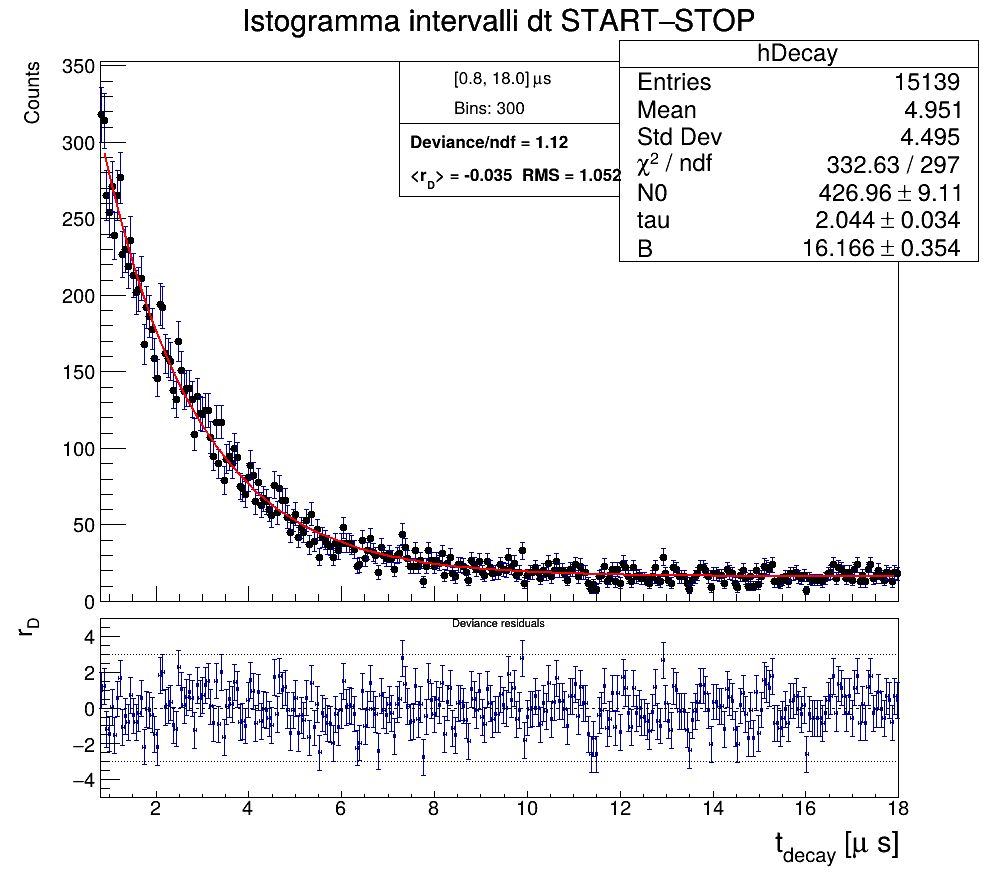
\includegraphics[width=\linewidth]{Grafici_fit_finale/mu_decay_fit_0.800_18.000_300_bins_withdevres.png}
        \caption{Risultati del fit realizzato con i nuovi parametri con annesso grafico dei residui}
        \label{fig:fit_final}
    \end{minipage}
    \hfill
    \begin{minipage}{0.48\linewidth}
        \centering
        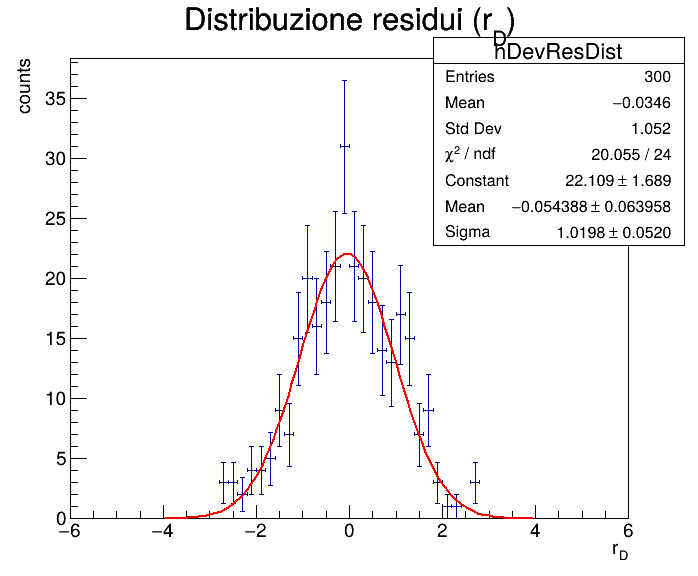
\includegraphics[width=\linewidth]{Grafici_fit_finale/devres_distribution_0.800_18.000_300_bins.png}
        \caption{Distribuzione dei residui per il fit finale}
        \label{fig:residui_2}
    \end{minipage}
\end{figure}
\end{flushleft}
Il fit restituisce un valore per vita media : $\bm{\tau = 2.044 \pm 0.034\mu}\textbf{s}$ e per gli altri parametri restituisce i valori $\bm{N_0=427 \pm 9 \textbf{ counts}}$ e $\bm{B= 16.2 \pm 0.3 \textbf{ counts}}$.\\
La distribuzione dei residui di devianza è ben approssimata da una gaussiana standard e non evidenzia problematiche, il valore medio $<r_{D}>=-0.035$ e $RMS=1.052$ favorisce l’ipotesi che, nell’intervallo $[t_{\min},t_{\max}]$ e con il modello adottati, le discrepanze osservate siano coerenti con fluttuazioni statistiche poissoniane.
Infine è stato calcolato il rapporto devianza su gradi di libertà ottenendo il risultato $D/ndof=1.12$ che non suggerisce particolari problemi nel nostro fit.\\


\newpage


\subsection{Misura del rapporto fra le popolazioni}\label{subsec:rapporto}
\begin{flushleft}
Abbiamo in seguito usato lo stesso set di dati per misurare l'abbondanza relativa fra muoni positivi e negativi. 

Per farlo abbiamo assunto nota la vita media del $\mu^{-}$ in carbonio (vedi sez.\ref{sec:intro}), ricavando così quella per il $\mu^{+}$: 

\begin{equation}
    \label{mean_life_tot}
    \tau = \frac{1}{2}(\tau_{+}+\tau_{-}) \implies \tau_{+} = 2\tau -\tau_{-}= 2.203 \mu \text{s}
\end{equation}

Dopodiché effettuiamo un fit con la funzione:

\begin{equation}
    \label{fit_func_2}
    g(t) = A_{+}e^{-\frac{t}{\tau_+}}+A_{-}e^{-\frac{t}{\tau_-}} + B
\end{equation}

I parametri in questo caso sono $A_{\pm}$ e $B$, mentre le vite medie ($\tau_+$ e $\tau_-$) sono fissate. Definiamo quindi due funzioni esponenziali con i parametri ottenuti dal fit precedente e ne calcoliamo l'integrale. Questo sarà proporzionale al numero di decadimenti per ciascuna carica $N_{\pm}$ in queso modo possiamo ricavare il rapporto tre le abbondanze nel seguente modo:\\
\begin{minipage}{0.45\linewidth}
\centering
\begin{equation}
    \label{height_muon}
    h_{\pm}(t) = A_{\pm}e^{-\frac{t}{\tau_{\pm}}}
\end{equation}
\end{minipage}
\hfill
\begin{minipage}{0.45\linewidth}
\centering
\begin{equation}
    \label{Number_muon}
    N_{\pm} =\int _{t_{min}}^{t_{max}}  A_{\pm}e^{-\frac{t}{\tau_{\pm}}} dt
\end{equation}
\end{minipage}\\
da cui:
\begin{equation}
    \label{Abbundancies}
    R = \frac{N_+}{N_-}
\end{equation}


L'area è stata trattata come una variabile poissoniana, di conseguenza l'errore associato a R può essere calcolato con la seguente relazione:
\begin{equation}
    \label{error_R}
    \sigma_R = R\sqrt{\frac{1}{N_+}+\frac{1}{N_-}}
\end{equation}
Utilizzando le relazioni \ref{Abbundancies} e \ref{error_R} otteniamo quindi $R = 1.07 \pm 0.08$

Il valore atteso è di 1.28 $\pm$ 0.32 (stats.) $\pm$ 0.32 (syst.)\footnote{\cite{CMSChargeRatio2010}}, compatibile con la nostra misura.
Il grafico del fit realizzato è stato riportato in appendice \ref{app:grafico_double}

\end{flushleft}
\section{Misura della massa del muone}\label{sec:misura_massa}

\subsection{Misura di spettro}\label{sec:misura_spettro}
\begin{flushleft}
Per la misura di massa del muone, è necessario ricostruire lo spettro in energia dell'elettrone emesso dal decadimento e individuare l'energia per cui si osserva un cut-off degli eventi.
Per effettuare la presa dati abbiamo utilizzato la scheda di acquisizione ADC in dotazione e un modulo integratore (per specifiche vedi sezione \ref{sec:apparato}).\\
Il modulo integratore è necessario in quanto effettuando l'integrale del segnale analogico proveniente dai PMT utilizzati, si ottiene una forma d'onda che tende a una step-funcion la cui altezza è direttamente proporzionale alla quantità di luce emessa nella lastra e di conseguenza ala quantità di energia rilasciata nel mezzo dalla particella.\\
Una volta eseguita l'operazione di integrazione, le uscite \textbf{OutL}\footnote{Uscita "bassa" cioè con costante di conversione più piccola $-0.83 mV/\text{pC}$ che permette di digitalizzare le forme d'onda senza saturare il digitizer} della scheda per ogni canale sono state collegate agli ingressi della scheda ADC per digitalizzare la forma d'onda ottenuta.\\
Per misurare lo spettro usiamo come trigger dell'acquisizione il segnale di STOP e impostiamo il programma\footnote{\texttt{Wavedump}} per registrare la forma d'onda in un intervallo di tempo $\Delta t\simeq10\mu \text{s}$ a seguito del trigger\footnote{Si possono modificare le impostazioni di acquisizione del programma \texttt{wavedump} modificando il file \texttt{wavedump\_config.txt} nel teminale}. La logica da noi implementata fa corrispondere ad ogni START uno STOP (non associato a un decadimento), dunque nella maggior parte dei casi\footnote{Le problematiche della logica implementata sono riportate nella sezione \ref{subsec:sys_err}} digitalizzeremo una forma d'onda non rappresentativa del processo di decadimento (singola step-function) ma del passaggio di un cosmico all'interno del mezzo. Gli eventi che noi desideriamo studiare sono quindi quelli a "doppio gradino" (vedi figura \ref{fig:step}) dovuti a un primo segnale di STOP e con un secondo picco riconducibile al decadimento del muone durante il ritorno a zero del segnale analogico del PMT\footnote{Da qui la tipica forma a "doppio gradino"}.\\
\newpage
Il primo gradino quindi corrisponde al muone entrato nel blocco, quindi la sua altezza è proporzionale all'energia del muone. L'altezza del secondo gradino invece è proporzionale alla somma dell'energia del muone e dell'elettrone. La differenza fra l'altezza dei due scalini è dunque proporzionale all'energia dell'elettrone. \\
\begin{figure}[H]
    \centering
    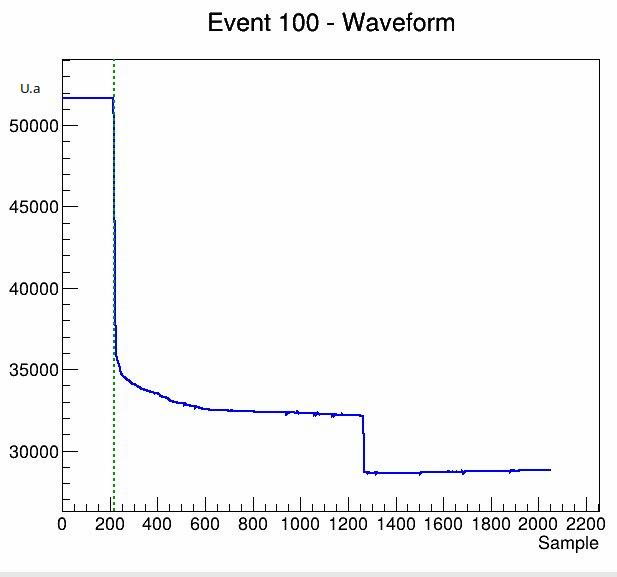
\includegraphics[width=0.5\linewidth]{Immagini/gradino.jpg}
    \caption{Esempio di forma d'onda digitalizzata}
    \label{fig:step}
\end{figure}
Prima di procedere con l'analisi delle forme d'onda digitalizzate è stato necessario calibrare la scheda ADC utilizzando come sorgente i raggi cosmici, questa procedura viene riportata in appendice \ref{appx:calib_adc}.\\
Per ricostruire lo spettro in energia degli elettroni di decadimento è stato realizzato un codice di analisi dati in \texttt{ROOT} che esegue in breve le seguenti istruzioni:

\begin{minipage}{0.45\linewidth}
\begin{itemize}
\item salva le forme d'onda campionate da ciascun canale (figura\ref{fig:step}) e le somma;
\item ne fa la derivata numerica(figura\ref{fig:deriv}), per la forma d'onda da noi analizzata corrisponde a una gaussiana localizzata nel punto di discesa approssimabile a un impulso di altezza proporzionale a quella dello scalino;
\item cerca eventi con due impulsi e ne salva le coordinate e altezza;
\item calcola l'energia moltiplicando la costante di calibrazione per l'altezza del secondo picco;
\item realizza un istogramma delle ampiezze.
\end{itemize}
\end{minipage}
\hfill
\begin{minipage}{0.48\linewidth}
\begin{figure}[H]
    \centering
    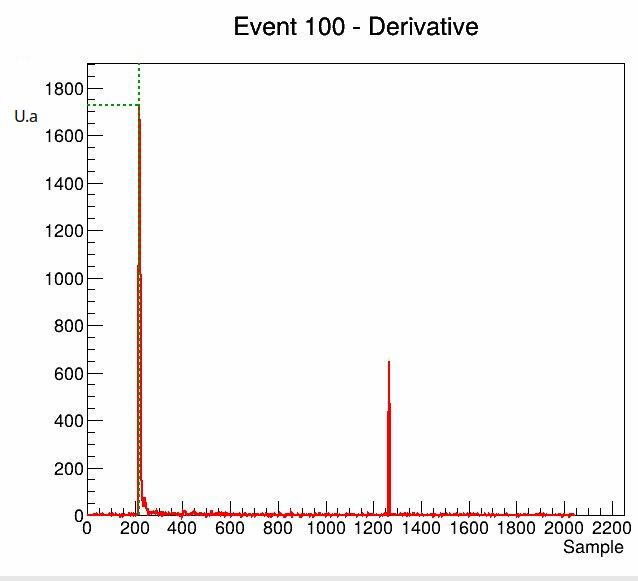
\includegraphics[width=1\linewidth]{Immagini/deriv.jpg}
    \caption{Esempio della derivata della forma d'onda digitalizzata}
    \label{fig:deriv}
\end{figure}
\end{minipage}

\newpage
Sono state quindi realizzate due prese dati (10/12-11/12 e 11/12-15/12) unendo i dataset e seguendo la procedura indicata in questa sezione, è stato quindi realizzato un istogramma dello spettro in energia degli elettroni di decadimento (figura\ref{fig:spettro})

\begin{figure}[H]
    \centering
    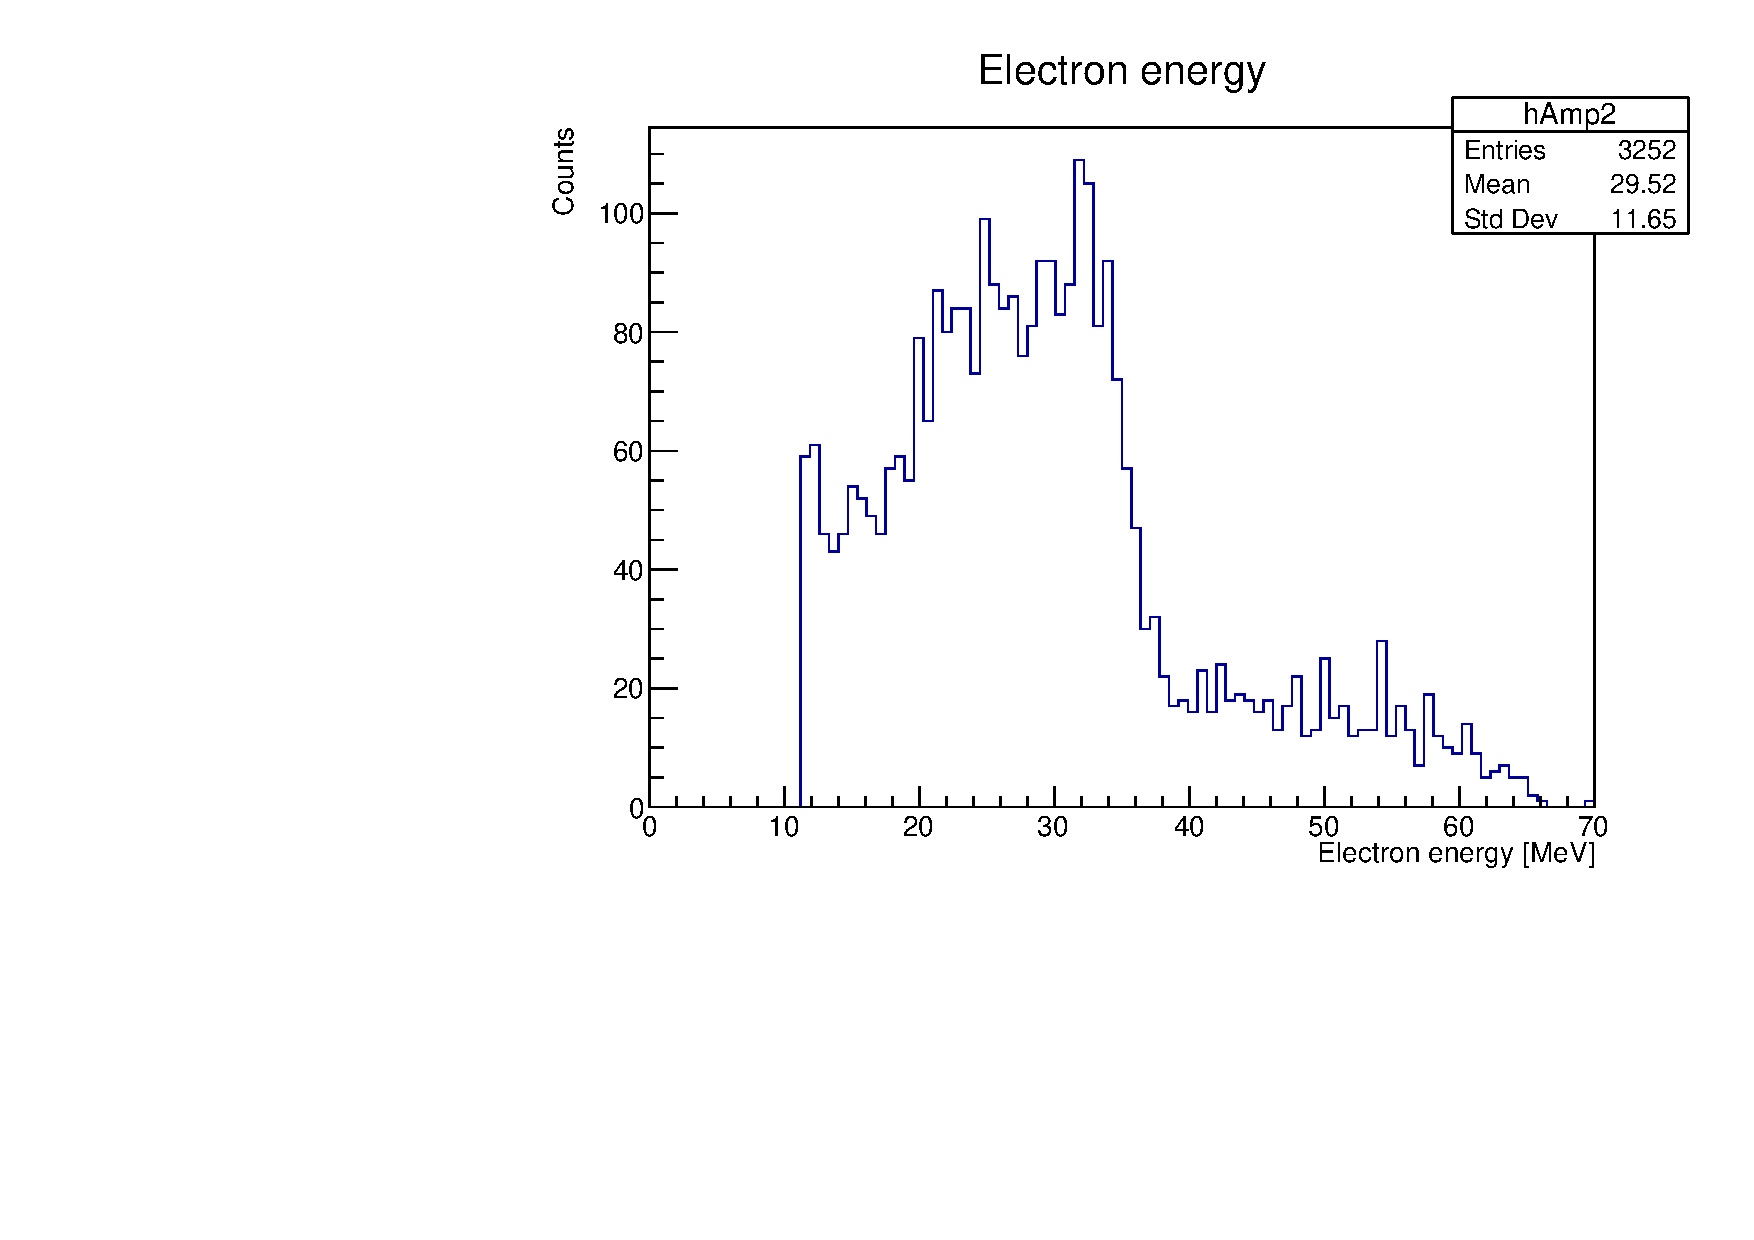
\includegraphics[width=0.5\linewidth]{Immagini/Spettro_Final.pdf}
    \caption{Istogramma delle energie degli elettroni di decadimento del muone}
    \label{fig:spettro}
\end{figure}
Come si può notare, l'end-point di questo spettro è distante circa 20 MeV dal valore di aspettazione di 52.8 MeV, inoltre vi è la presenza di una coda successivamente al massimo che a livello cinematico non è consentita dovuta a un fondo non eliminabile. Pertanto dall'analisi dello spettro individuando il cut-off $\simeq 40\text{M}eV$ la stima della massa del muone risulta  $m_{\mu_{misura}}\simeq 80\text{M}eV$.

\end{flushleft}

\section{Conclusioni}\label{sec:conclusion}
Grazie ai dati acquisiti è stato possibile misurare la vita media del muone all'interno dello scintillatore plastico (approssimabile a carbonio) ottendo il risultato di $\bm{\tau = 2.044 \pm 0.034\mu}\textbf{s}$, questo valore se confrontato con quello di sezione \ref{sec:intro} ($\tau_{\mu_{cabon}}=2.099 \pm 0.006$) risulta compatibile entro $2\sigma$, il fit realizzato in sezione \ref{subsec:fit_final} non mostra particolari problematiche e gli indicatori utilizzati non evidenziano criticità.\\
Per quanto riguarda la misura del rapporto di popolazione $R = 1.07 \pm 0.08$ il valore ottenuto risulta compatibile con il valore riportato in sezione \ref{subsec:rapporto} anceh se il grafico del fit realizzato (figura \ref{fig:fit_double_graph}) mostra un andamento dei residui sospetto che fa ipotizzare uno scarso accordo del modello utilizzato con i dati sperimentali.
Per quanto riguarda la misura della massa del muone tramite lo spettro degli elettroni di decadimento, il risultato ottenuto non è compatibile con la massa del muone. Lo spettro ricreato in figura \ref{fig:spettro} tuttavia presenta le caratteristiche che ci si potrebbe aspettare da questo fenomeno al netto di un'energia di cut-off sottostimata e un fondo statistico non previsto per alte energie. Questa discrepanza potrebbe essere dovuta all'impossibilità di digitalizzare completamente alcune forme d'onda da parte del digitizer, durante l'acquisizione ci siamo resi conto che molto spesso questo saturava e non mostrava l'ampiezza totale del secondo "scalino" nella forma d'onda. Questo problema potrebbe essere ovviato utilizzando un'unità per attenuare il segnale in uscita dai vari PMT per fare in modo di digitalizzare l'intera forma d'onda. Altra ipotesi potrebbe essere una errata calibrazione del fattore di conversione (vedi appendice \ref{appx:calib_adc}) dovuta a non abbastanza statisca o errori di conversione.\\


\newpage
\section{Bibliografia}
% --- Bibliografia manuale (senza BibTeX) ---
\begin{thebibliography}{99}

\bibitem{CMSChargeRatio2010}
CMS Collaboration,
\textit{Measurement of the charge ratio of atmospheric muons with the CMS detector},
Physics Letters B \textbf{692} (2010) 83--104.
doi:\ 10.1016/j.physletb.2010.07.033.
arXiv:\ 1005.5332 [hep-ex].

\bibitem{GasparikSivertzNSRL2023}
J.~Gasparik and M.~Sivertz,
\textit{Muon Decay Study at NSRL},
Brookhaven National Laboratory (BNL), Technical Report (Mar 2023).
Report no.\ BNL-224196-2023-TECH, NSRL-TN-23-001.
doi:\ 10.2172/1968830.
Available at:\ \url{https://www.osti.gov/biblio/1968830} (accessed 2026-01-31).

\bibitem{PDG2024}
S.~Navas et al.\ (Particle Data Group),
\textit{Review of Particle Physics},
Physical Review D \textbf{110} (2024) 030001.
doi:\ 10.1103/PhysRevD.110.030001.

% (Opzionale) se vuoi citare esplicitamente la pagina/listing del muone
\bibitem{PDG2024MuonListing}
Particle Data Group,
\textit{Muon (Particle Listings), in Review of Particle Physics (2024)},
\url{https://pdgaws.lbl.gov/2024/listings/rpp2024-list-muon.pdf}
(accessed 2026-01-31).

\end{thebibliography}


\newpage
\appendix
\section{Tabelle dati efficienza PMT del bersaglio}
\label{app:target}
Riportiamo le tabelle utilizzate per la realizzazione del grafico \ref{fig:target}
\begin{table}[H]
    \begin{minipage}{0.45\linewidth}
        \centering
        \resizebox{0.8\linewidth}{!}{    \begin{tabular}{cccc}
    \toprule
    HV [V] ($\pm$ 1 V)& $\varepsilon [\%]$ & $\sigma_{\varepsilon} [\%]$ & $D_{fake}$ \\
    \midrule
    1100 & 76 & $\pm$ 2 & 0.01 \\
    1130 & 81 & $\pm$ 2 & 0.02 \\
    1150 & 80 & $\pm$ 2 & 0.02 \\
    1175 & 74 & $\pm$ 2 & 0.03 \\
    1200 & 82 & $\pm$ 2 & 0.04 \\
    1230 & 82 & $\pm$ 2 & 0.06 \\
    1250 & 78 & $\pm$ 2 & 0.07 \\
    \bottomrule
    \end{tabular}}
        \caption{PMT08}
        \label{tab:PMT08}
    \end{minipage}
    \hfill
    \begin{minipage}{0.45\linewidth}
        \centering
        \resizebox{0.8\linewidth}{!}{    \begin{tabular}{cccc}
    \toprule
    HV [V] ($\pm$ 1V) & $\varepsilon [\%]$ & $\sigma_{\varepsilon} [\%]$ & $D_{fake}$ \\
    \midrule
    1100 & 75 & $\pm$ 2 & 0.080 \\
    1130 & 76 & $\pm$ 2 & 0.076 \\
    1170 & 76 & $\pm$ 2 & 0.077 \\
    1200 & 81 & $\pm$ 2 & 0.077 \\
    1230 & 78 & $\pm$ 2 & 0.078 \\
    1250 & 77 & $\pm$ 2 & 0.079 \\
    1277 & 84 & $\pm$ 2 & 0.077 \\
    1300 & 86 & $\pm$ 2 & 0.079 \\
    \bottomrule
    \end{tabular}}
        \caption{PMT09}
        \label{tab:PMT09}
    \end{minipage}
    \hfill
\end{table}
\begin{table}[H]
    \begin{minipage}{0.45\linewidth}
        \centering
        \resizebox{0.8\linewidth}{!}{    \begin{tabular}{cccc}
    \toprule
    HV [V] ($\pm$ 1V) & $\varepsilon [\%]$ & $\sigma_{\varepsilon} [\%]$ & $D_{fake}$ \\
    \midrule
    1070 & 53 & $\pm$ 5 & 0.054 \\
    1100 & 60 & $\pm$ 5 & 0.047 \\
    1150 & 64 & $\pm$ 4 & 0.055 \\
    1170 & 56 & $\pm$ 5 & 0.054 \\
    1200 & 56 & $\pm$ 5 & 0.059 \\
    1230 & 59 & $\pm$ 5 & 0.054 \\
    \bottomrule
    \end{tabular}}
        \caption{PMT10}
        \label{tab:PMT10}
    \end{minipage}
    \hfill
    \begin{minipage}{0.45\linewidth}
        \centering
        \resizebox{0.8\linewidth}{!}{\begin{tabular}{cccc}
    \toprule
    HV [V] ($\pm$ 1V) & $\varepsilon [\%]$ & $\sigma_{\varepsilon} [\%]$ & $D_{fake}$ \\
    \midrule
    1100 & 74 & $\pm$ 2 & 0.077 \\
    1130 & 76 & $\pm$ 2 & 0.077 \\
    1170 & 76 & $\pm$ 2 & 0.077 \\
    1200 & 81 & $\pm$ 2 & 0.077 \\
    1230 & 78 & $\pm$ 2 & 0.077 \\
    1250 & 79 & $\pm$ 2 & 0.079 \\
    1277 & 84 & $\pm$ 2 & 0.080 \\
    1300 & 86 & $\pm$ 2 & 0.079 \\
    \bottomrule
\end{tabular}}
        \caption{PMT11}
        \label{tab:PMT11}
    \end{minipage}
    \hfill
\end{table}
\newpage
\section{Stima dell'accettanza dal Montecarlo}
\label{aapx:montecarlo}
\begin{flushleft}
Per stimare l'accettanza $A$ è necessario stimare la probabilità che un raggio cosmico attraversi il rivelatore dato il passaggio per gli altri due. Tale valore viene poi usato per stimare l'efficienza tramite:

\begin{equation}
\label{eq:eff}
\varepsilon = \frac{1}{A}\frac{\#(1\land 2\land 3)}{\#(1\land 2)}
\end{equation}

dove $\#(1\land 2\land 3)$ è il numero di triple e $\#(1\land 2)$ quello di doppie misurato. 

Per stimare tale parametro è stato realizzato un \textit{toy monte-carlo} in \texttt{ROOT} che genera traiettorie di raggi cosmici in accordo con la distribuzione angolare:

\begin{equation}
\label{eq:cosmic_dist}
f(\theta, \phi) \propto cos^{2}(\theta)
\end{equation}

dove $\theta$ è l'angolo azimutale, $\phi$ quello polare. L'intercetta è generata come punto distribuito uniformemente entro la superficie del rivelatore posto a $z=0$. Per completezza, mostriamo un istogramma bidimensionale delle intercette nei piani superiori e inferiori:

\begin{figure}[H]
    \centering
    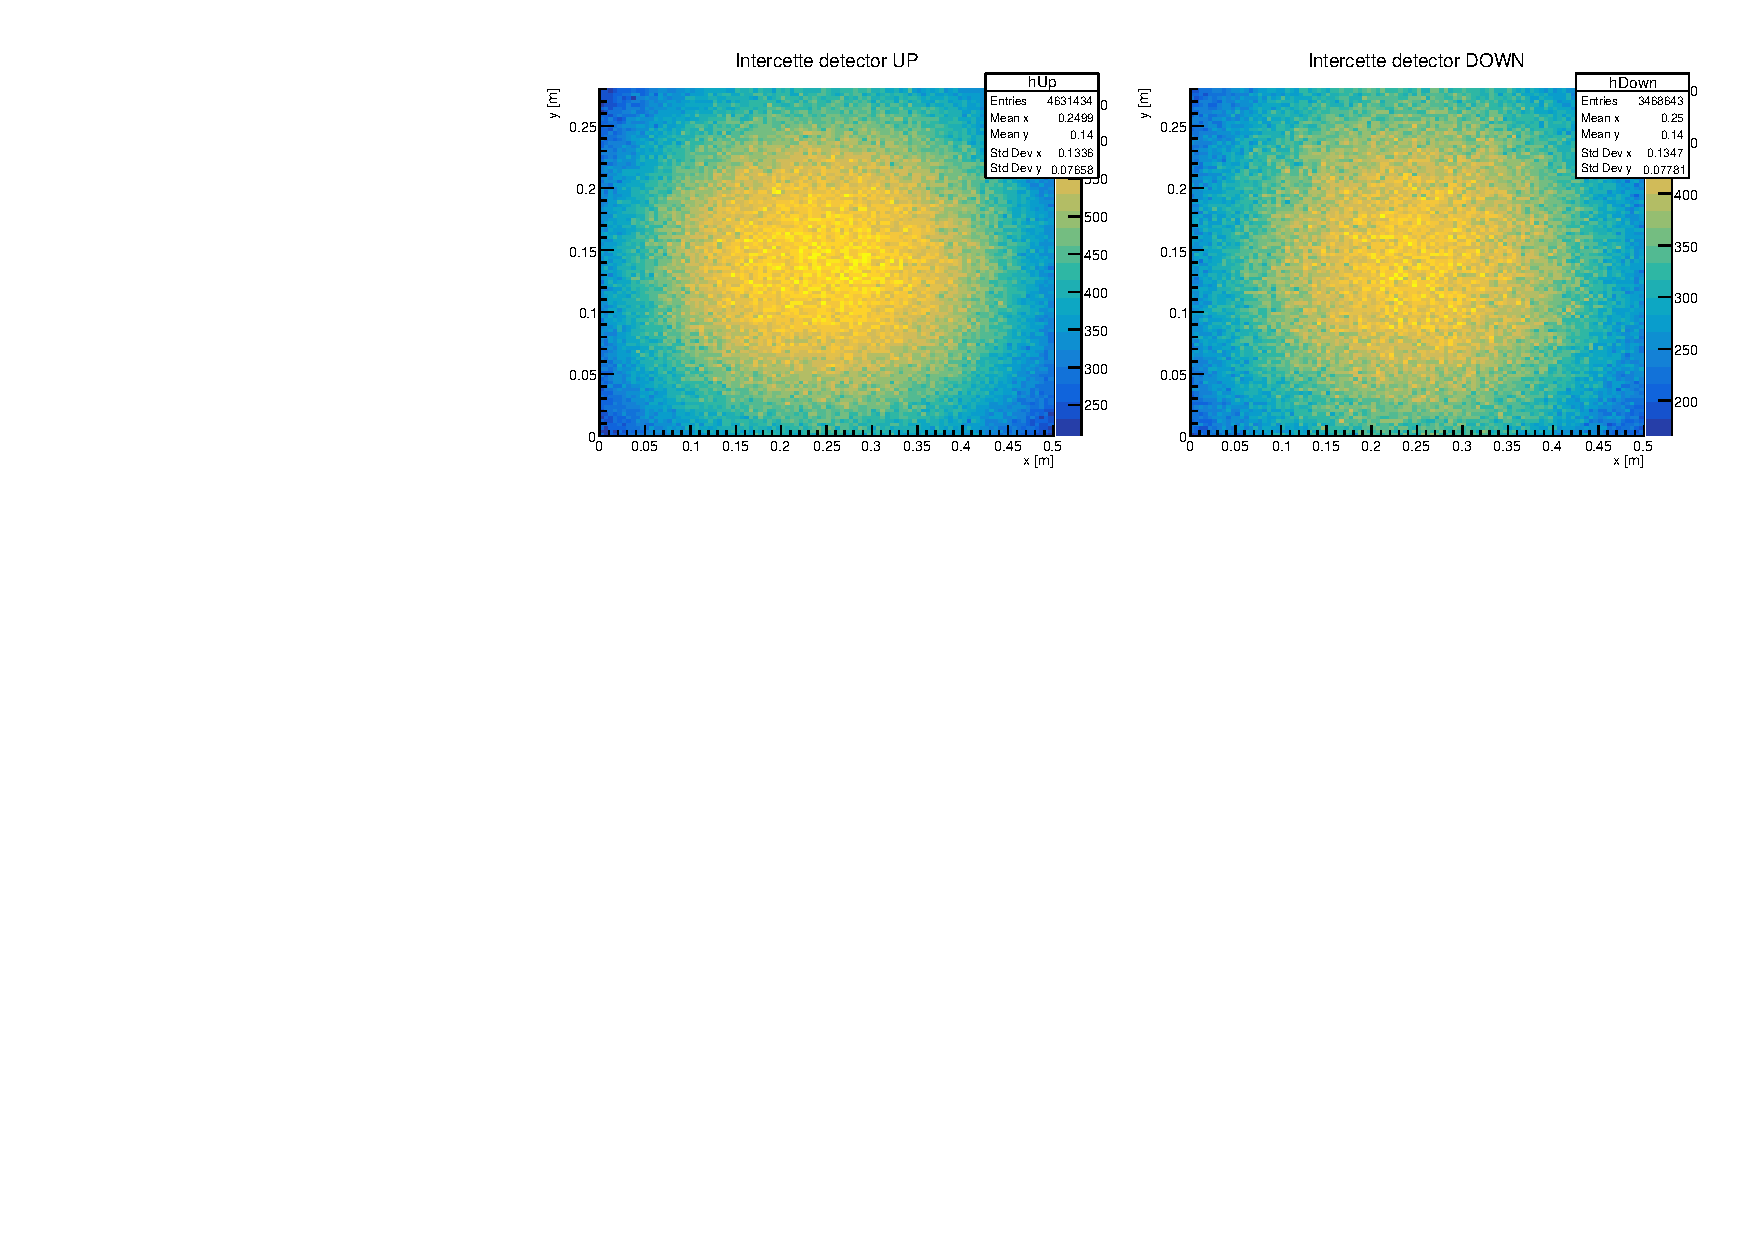
\includegraphics[width=0.75\linewidth]{Grafici/MCplot.pdf}
    \caption{Grafico delle intercette nei piani dei rilevatori superiori e inferiori}
    \label{fig:montecarlo}
\end{figure}

Il codice poi conta il numero di raggi cosmici passati attraverso due e tre rivelatori. Da questi otteniamo: 

\begin{equation}
\label{eq:accettanza}
A = \frac{N_{1\land2\land3}}{N_{1\land2}}
\end{equation}

usata per poter stimare l'efficienza coerentemente con la geometria del sistema.

\end{flushleft}
\newpage
\section{Calcolo per la configurazione ottimale per il PMT10}
\label{app:target_PMT10}
\begin{flushleft}
    
Per ottenere la configurazione ottimale per la misura di efficienza per il PMT10 e 01 abbiamo ragionato nel seguente modo. In primis, riportiamo una bozza della geometria di riferimento vista per sezione:

\begin{figure}[H]
    \centering
    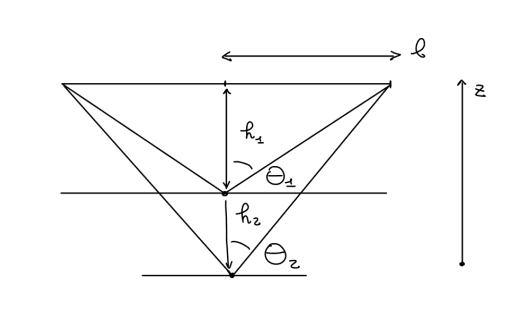
\includegraphics[width=0.5\linewidth]{Immagini/Geometria.png}
    \caption{Schema dell'apparato}
    \label{fig:geometria_PMT10}
\end{figure}

le due linee superiori sono le lastre di scintillatore mentre la linea inferiore rappresenta il blocco. Per calcolare la probabilità del passaggio per tutti e tre i rivelatori (evento $B$) dato quello per i due PMT (evento $A$) usiamo :

\begin{equation}
P(B|A) = \frac{P(B\cap A)}{P(A)}
\end{equation}

Interpretiamo $A$ come passaggio della traiettoria entro l'angolo solido di apertura $\theta_1$, mentre $B$ come passaggio entro quello di apertura $\theta_2$. Inoltre, essendo $\theta_2<\theta_1$, $B\cap A = B$.

Nota la distribuzione angolare dei raggi cosmici $f(\theta, \phi)$ (eq. \ref{eq:cosmic_dist}) avrò dunque:

\begin{equation}
P(B|A) = \frac{\int^{2\pi}_{0}{d\phi}\int^{\theta_2}_{0}d\theta f(\theta,\phi)}{\int^{2\pi}_{0}{d\phi}\int^{\theta_1}_{0}d\theta f(\theta,\phi)}
\end{equation}
segue
\begin{equation}
\label{eq:probab_comsic}
P(B|A) = \frac{1-cos^{3}(\theta_2)}{1-cos^{3}(\theta_1)}
\end{equation}

dove $\theta_1$ e $\theta_2$ sono gli angoli massimi accettati da telescopio e bersaglio come visibile in figura \ref{fig:geometria_PMT10}.\\
Dalla relazione \ref{eq:probab_comsic} si evince che la condizione che massimizza tale probabilità è $\theta_1\rightarrow0$, con $\theta_1\approx \frac{l}{D}$, $l$ la larghezza dello scintillatore e $D$ la distanza fra lo stesso e il bersaglio. Dunque massimizzando $D$ si aumenta la probabilità, da cui la scelta dei PMT08/07.
\newpage
\end{flushleft}
\section{Logica del programma}
\label{app:logica_prog_1}
\begin{flushleft}
La scheda di sviluppo DEO10-NANO si interfaccia al computer con un programma di acquisizione da terminale chiamato \texttt{./FIFOread}, questo una volta terminata l'acquisizione restituisce un file txt contenente gli eventi registrati.\\ Nel file restituito sono presenti due colonne una che indica i canali attivi al momento della digitalizzazione e l'altra che mostra il numero di cicli di clock passati dall'inizio dell'acquisizione.\\ Ogni $2^{30}$ cicli di clock si visualizzerà una parola di reset $2147483648=2^{31}$ questa indica che il contatore si è resettato e il successivo ciclo di acquisizione è iniziato, nella seconda colonna troviamo $2147483648 +n_i$ dove $n_i$ indica il numero di reset effettuati. A seguito del reset il numero di cicli di clock viene registrato di nuovo a partire da zero.\\
Durante l'acquisizione i vari canali di input connessi alla scheda vengono segnalati nella digitalizzazione come una potenza di 2, nel nostro caso la codifica di ogni segnale registrato sarà la seguente:
\begin{itemize}
    \item START $\rightarrow$ CH0 $\rightarrow$ $2^0=1$
    \item STOP $\rightarrow$ CH1 $\rightarrow$ $2^1=2$
    \item 08 $\rightarrow$ CH2 $\rightarrow$ $2^2=4$
    \item 09 $\rightarrow$ CH3 $\rightarrow$ $2^3=8$
    \item 10 $\rightarrow$ CH4 $\rightarrow$ $2^4=16$
    \item 11 $\rightarrow$ CH5 $\rightarrow$ $2^5=32$
\end{itemize}
Quindi ad esempio se la scheda registrasse contemporaneamente segnale su CH1+CH2+CH4 vedremo nella colonna del file un numero pari alla somma in potenze di 2, in questo caso 2+4+16=22 .\\
Questa codifica è stata fondamentale nella realizzazione della logica del codice \texttt{ROOT} realizzato in quanto ha permesso di filtrare gli STOP generati a seguito di uno START, di determinare da quale PMT provenisse il segnale di START (approssimativamente dove si è fermato il muone) e infine di identificare in quale PMT hanno prodotto segnale gli elettroni di decadimento.\\
Il codice da noi progettato implementa una logica di pairing START-STOP che funziona in questo modo:
\begin{itemize}
    \item Individua uno START (rappresentato da un 1 nella prima colonna)
    \item individua lo STOP legato allo START sempre presente data la logica dei segnali (sez.\ref{subsec:logica_segnali}), tipicamente questo primo STOP si trova entro 50ns dal primo segnale(osservato all'oscilloscopio) quindi si inserisce come condizione la ricerca in questo arco temporale 
    \item nel caso lo STOP sia sovrapposto a un segnale del blocco annota da quale blocco proviene lo STOP e quindi lo START (ricerca una qualsiasi combinazione 2+4,2+8,2+16 ecc..)
    \item nel caso non fosse così, nell'intorno di $\pm 2\text{clock tick}$ centrato nello STOP cerca un segnale proveniente dai PMT del bersaglio e lo annota
    \item a partire dallo START ricerca un segnale di STOP entro 20$\mu $s e nel caso fosse sovrapposto al segnale di uno o più PMT annota quale lo ha generato
    \item altrimenti si ricerca nell'intorno di $\pm 3\text{clock tick}$ un segnale di questi PMT e lo annota (ricerca tutte le combinazioni 4,8,16,4+8,4+16,...)
    \item se tutto è andato bene effettua il pairing START-STOP, calcola il $dt$ e lo inserisce in un istogramma 
\end{itemize}
Oltre a questo nel programma sono presenti la gestione delle parole di reset e la realizzazione dell'istogramma per ogni PMT del quale non approfondiamo la logica.\\





    
\end{flushleft}

\newpage
\section{Calibrazione DEO10-nano}\label{app:Calib_deo}
\begin{flushleft}
Per acquisire i tempi di decadimento usiamo la scheda di sviluppo DEO10-nano. A questa sono stati collegati in input (ne ha 10 in totale) i nostri segnali dopo una conversione da logica NIM a logica TTL. L'output restituito dalla scheda è un file che contiene il canale in cui ha registrato il segnale e l'istante temporale riportato come numero di cicli di clock passati dall'inizio del conteggio. 

Per avere una misura di tempo è dunque necessaria un'opportuna calibrazione che converta il singolo tick di clock in un istante temporale.
Per fare ciò, usiamo la funzione End Marker di un'unità di timer per mandare un segnale a una seconda, la cui uscita viene mandata di nuovo alla prima. Questo causa un auto-oscillazione che genera un'onda quadra, di parametri (frequenza e duty cycle) personalizzabili modulando la lunghezza dell'impulso.
Confrontando la lettura della scheda con la frequenza dell'onda quadra misurata all'oscilloscopio possiamo ottenere la costante di calibrazione.\\
\begin{minipage}{0.44\textwidth}
Mandando in input l'onda quadra al DEI10-nano abbiamo acquisito dei punti e calcoliamo la differenza temporale in digit. Facendo questa operazione varie volte otteniamo una distribuzione, da questa stimiamo dunque il periodo in digit come la media della distribuzione e l'errore associato con la deviazione standard della media. 
\end{minipage}
\hfill
\begin{minipage}{0.44\textwidth}
\begin{figure}[H]
    \centering
    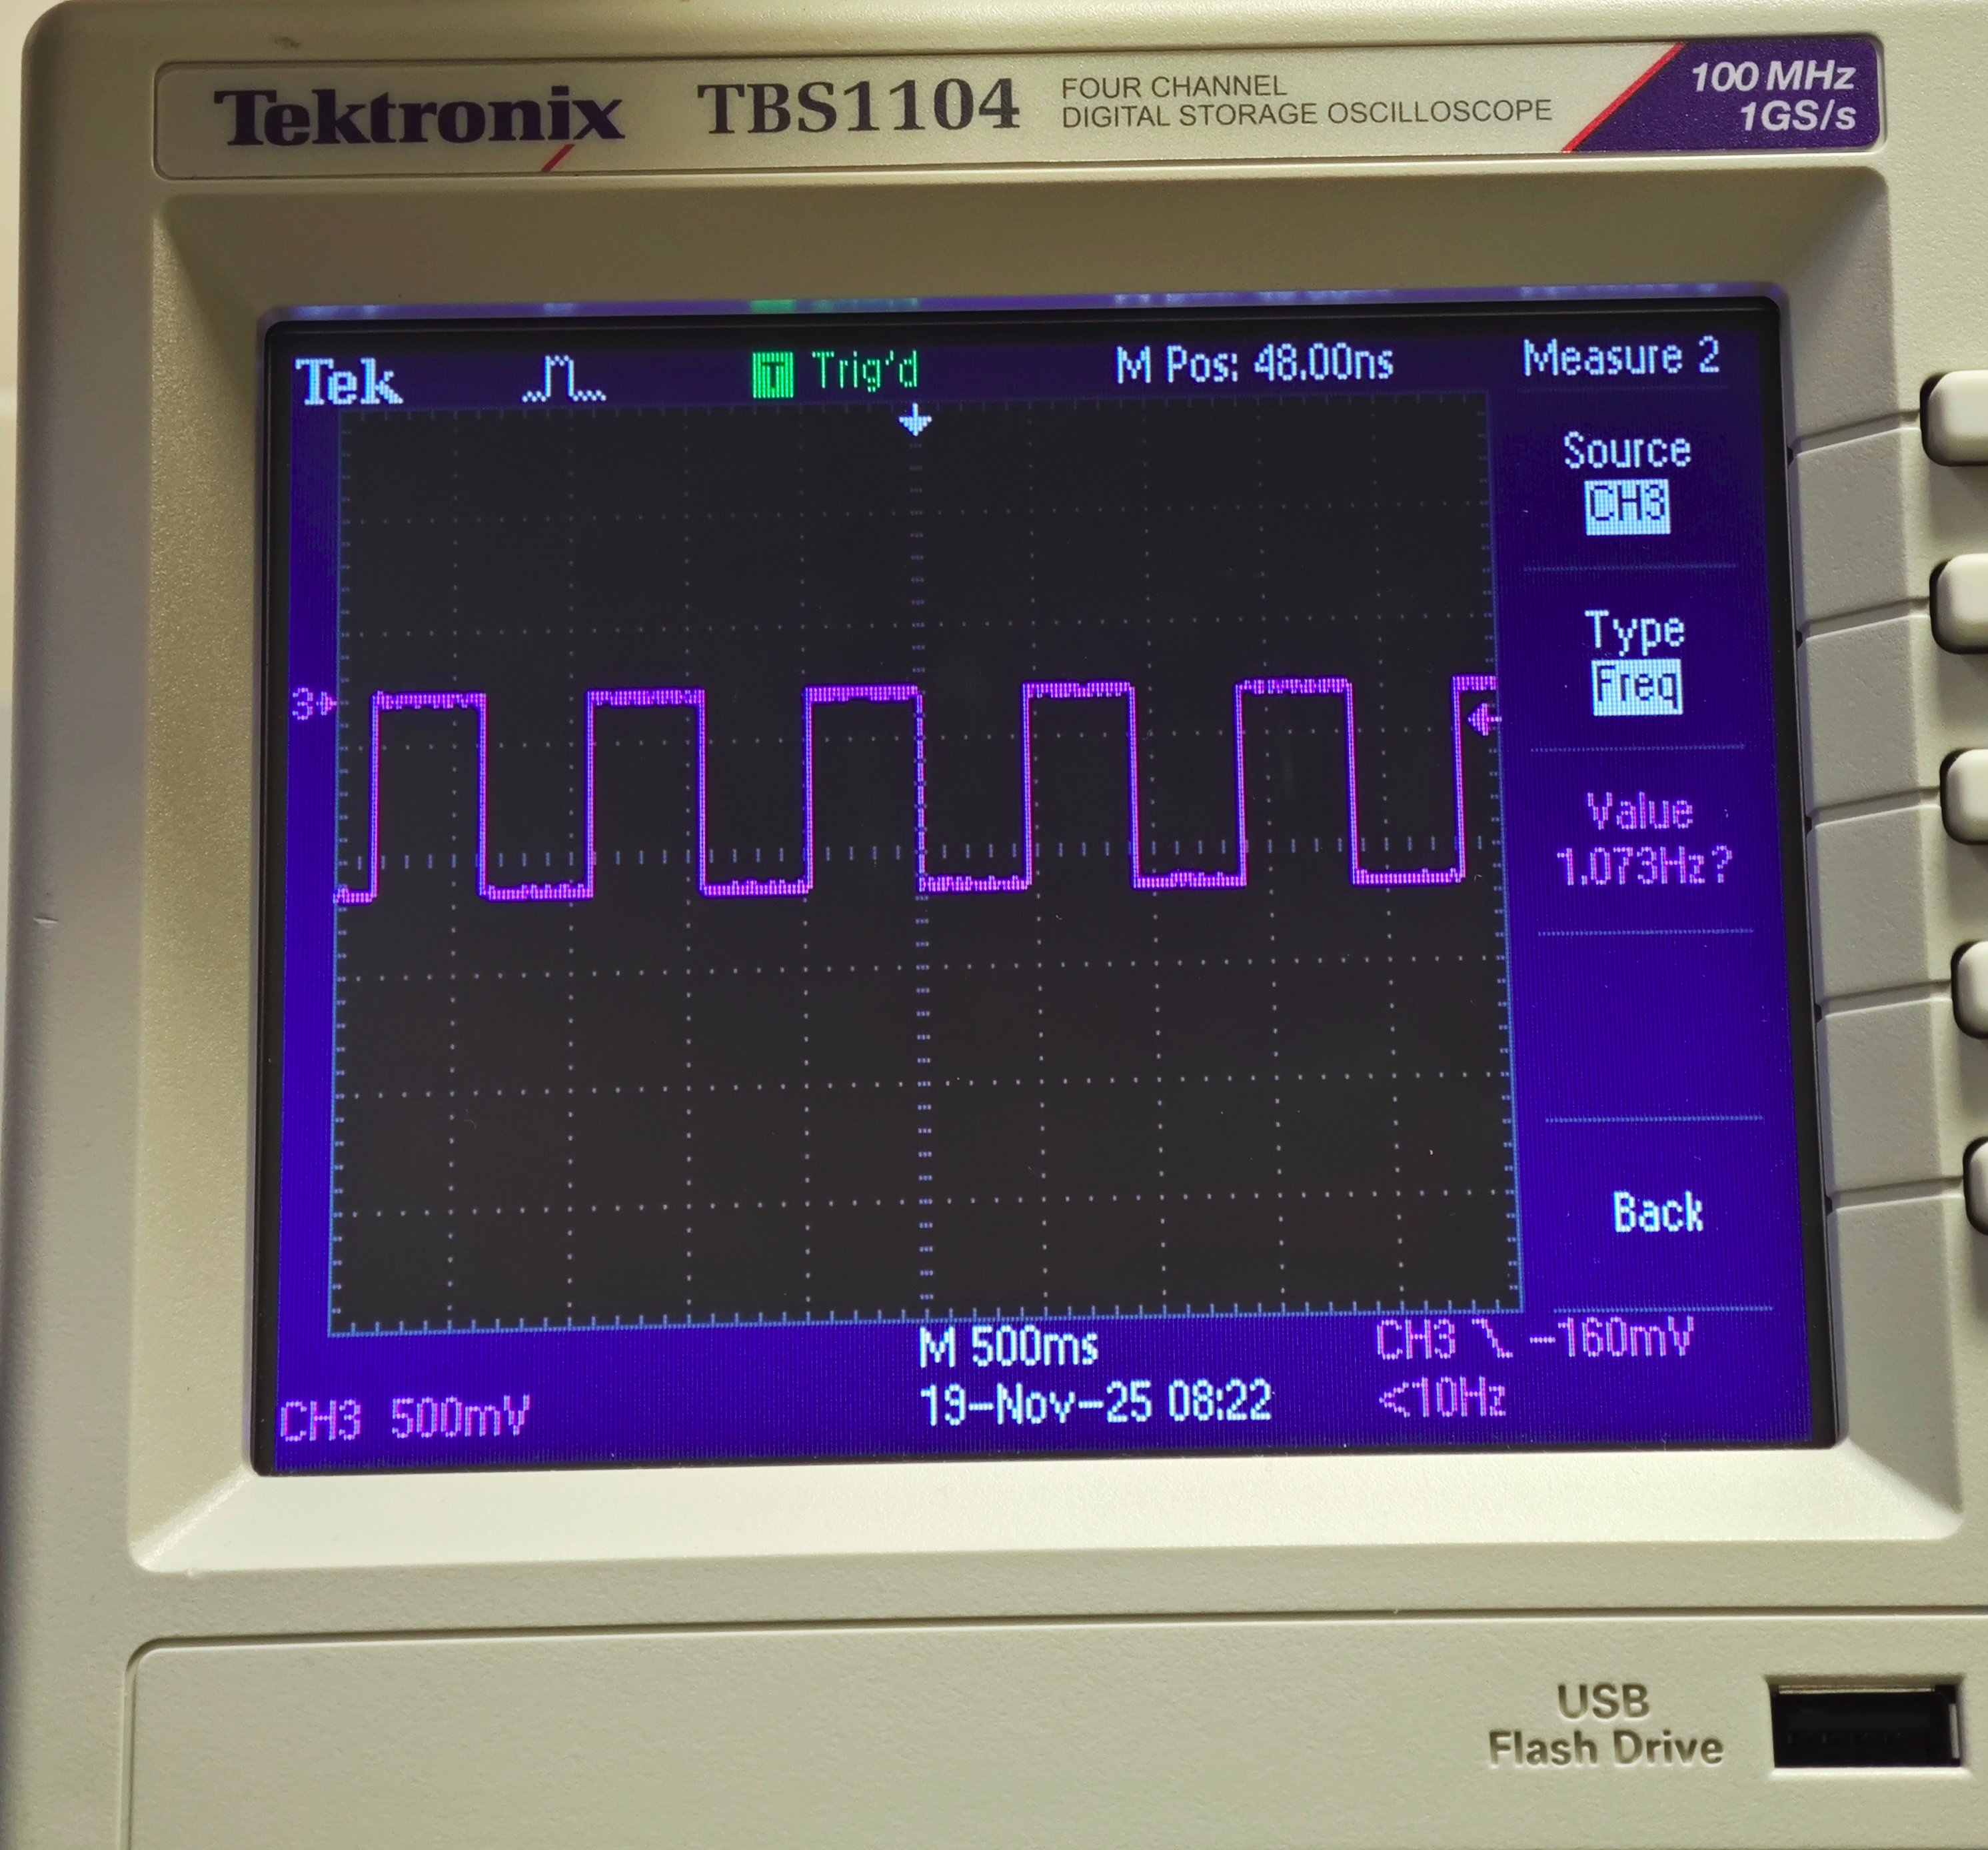
\includegraphics[width=0.8\linewidth]{Immagini/Onda_calib.jpg}
    \caption{Onda quadra generata dalle unità dual timer utilizzata frequenza $\nu= 1.071\text{Hz}$}
    \label{fig:onda_calib}
\end{figure}
\end{minipage}
\vspace{0.7cm}\\
Per completezza abbiamo misurato anche il ritardo fra due canali (lo 0 e l'1), mandando due onde quadre in fase fra loro per vedere se vi era un ritardo dovuto all'acquisizione.
Riportiamo di seguito due grafici con le nostre misure:

\begin{figure}[H]
\centering
    \begin{minipage}{0.4\textwidth}
        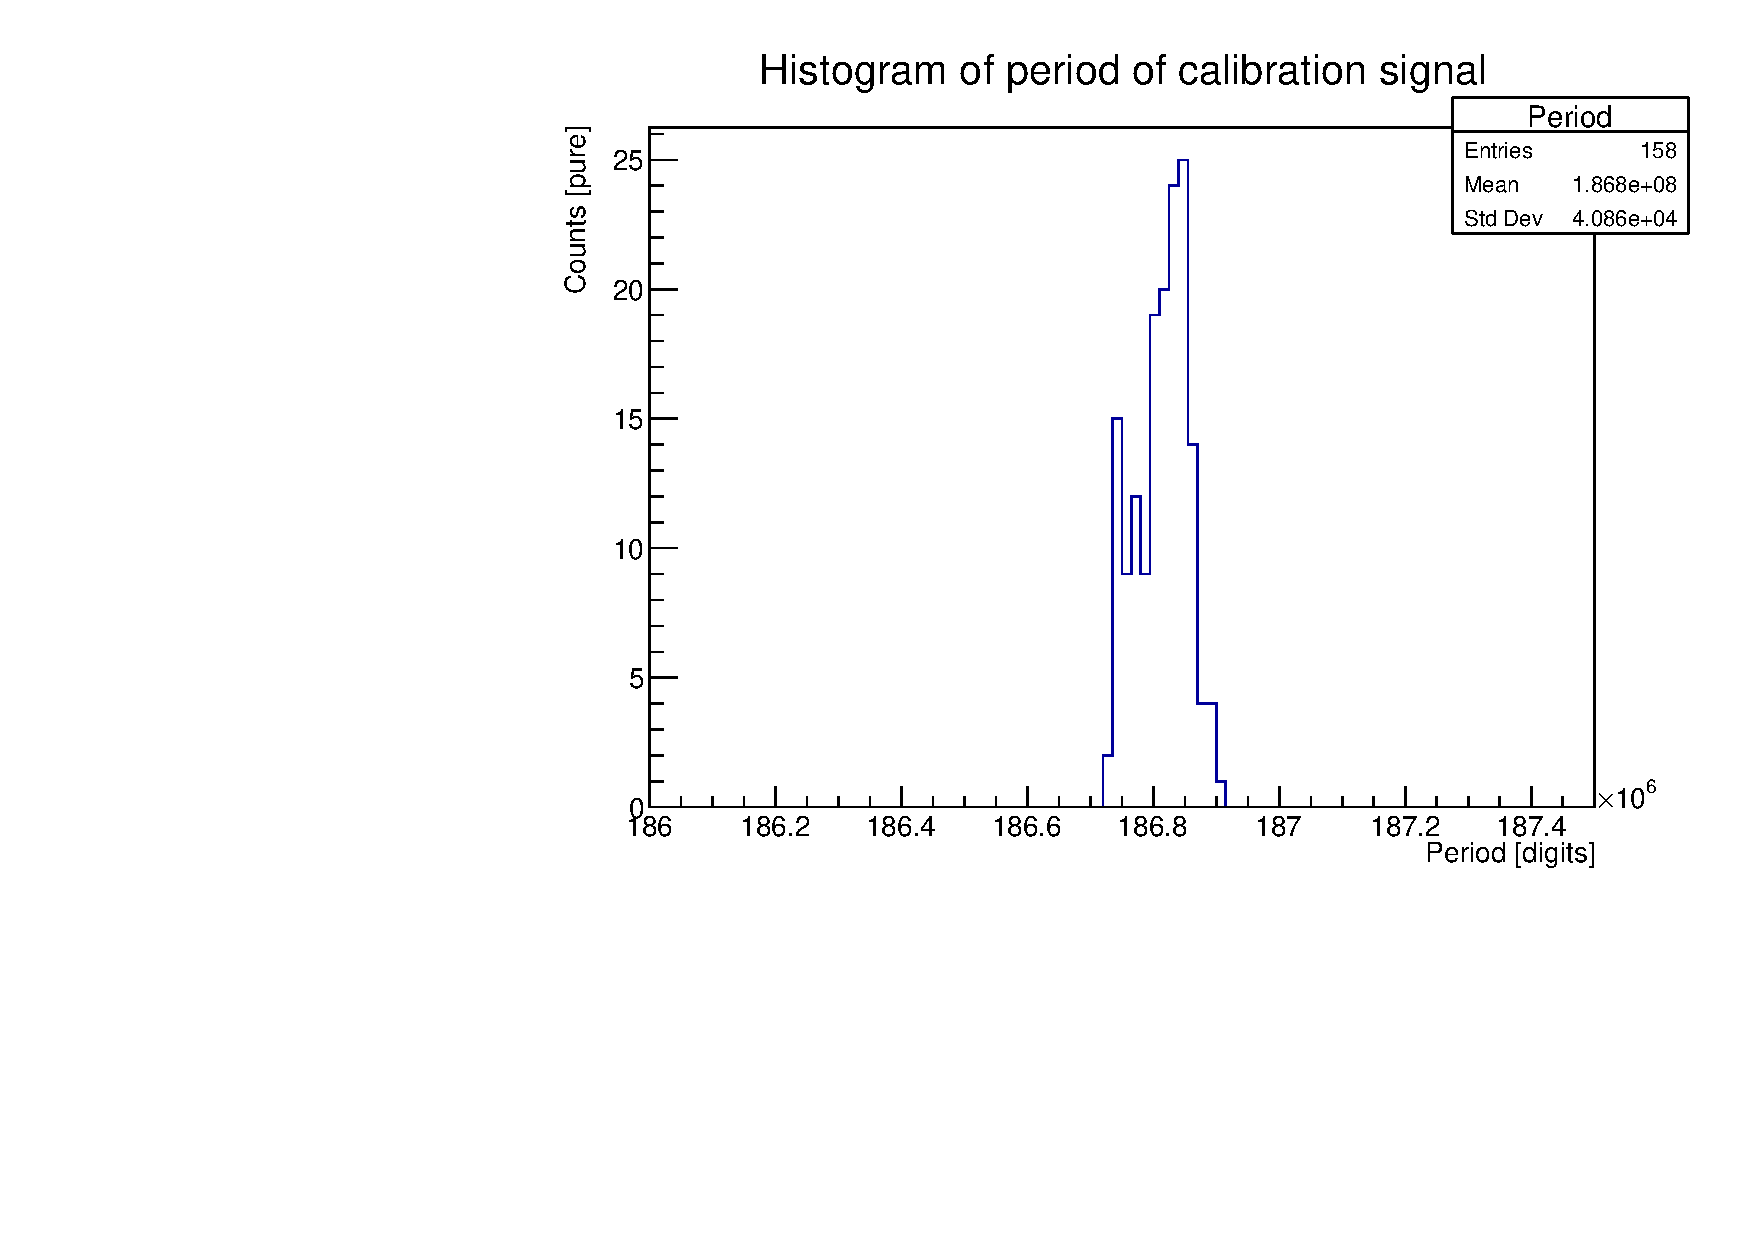
\includegraphics[width=\linewidth]{Grafici/Periodo.pdf}
        \caption{Periodi misurati per il segnale di calibrazione}
        \label{fig:period_NANO}
    \end{minipage}
    \begin{minipage}{0.5\textwidth}
        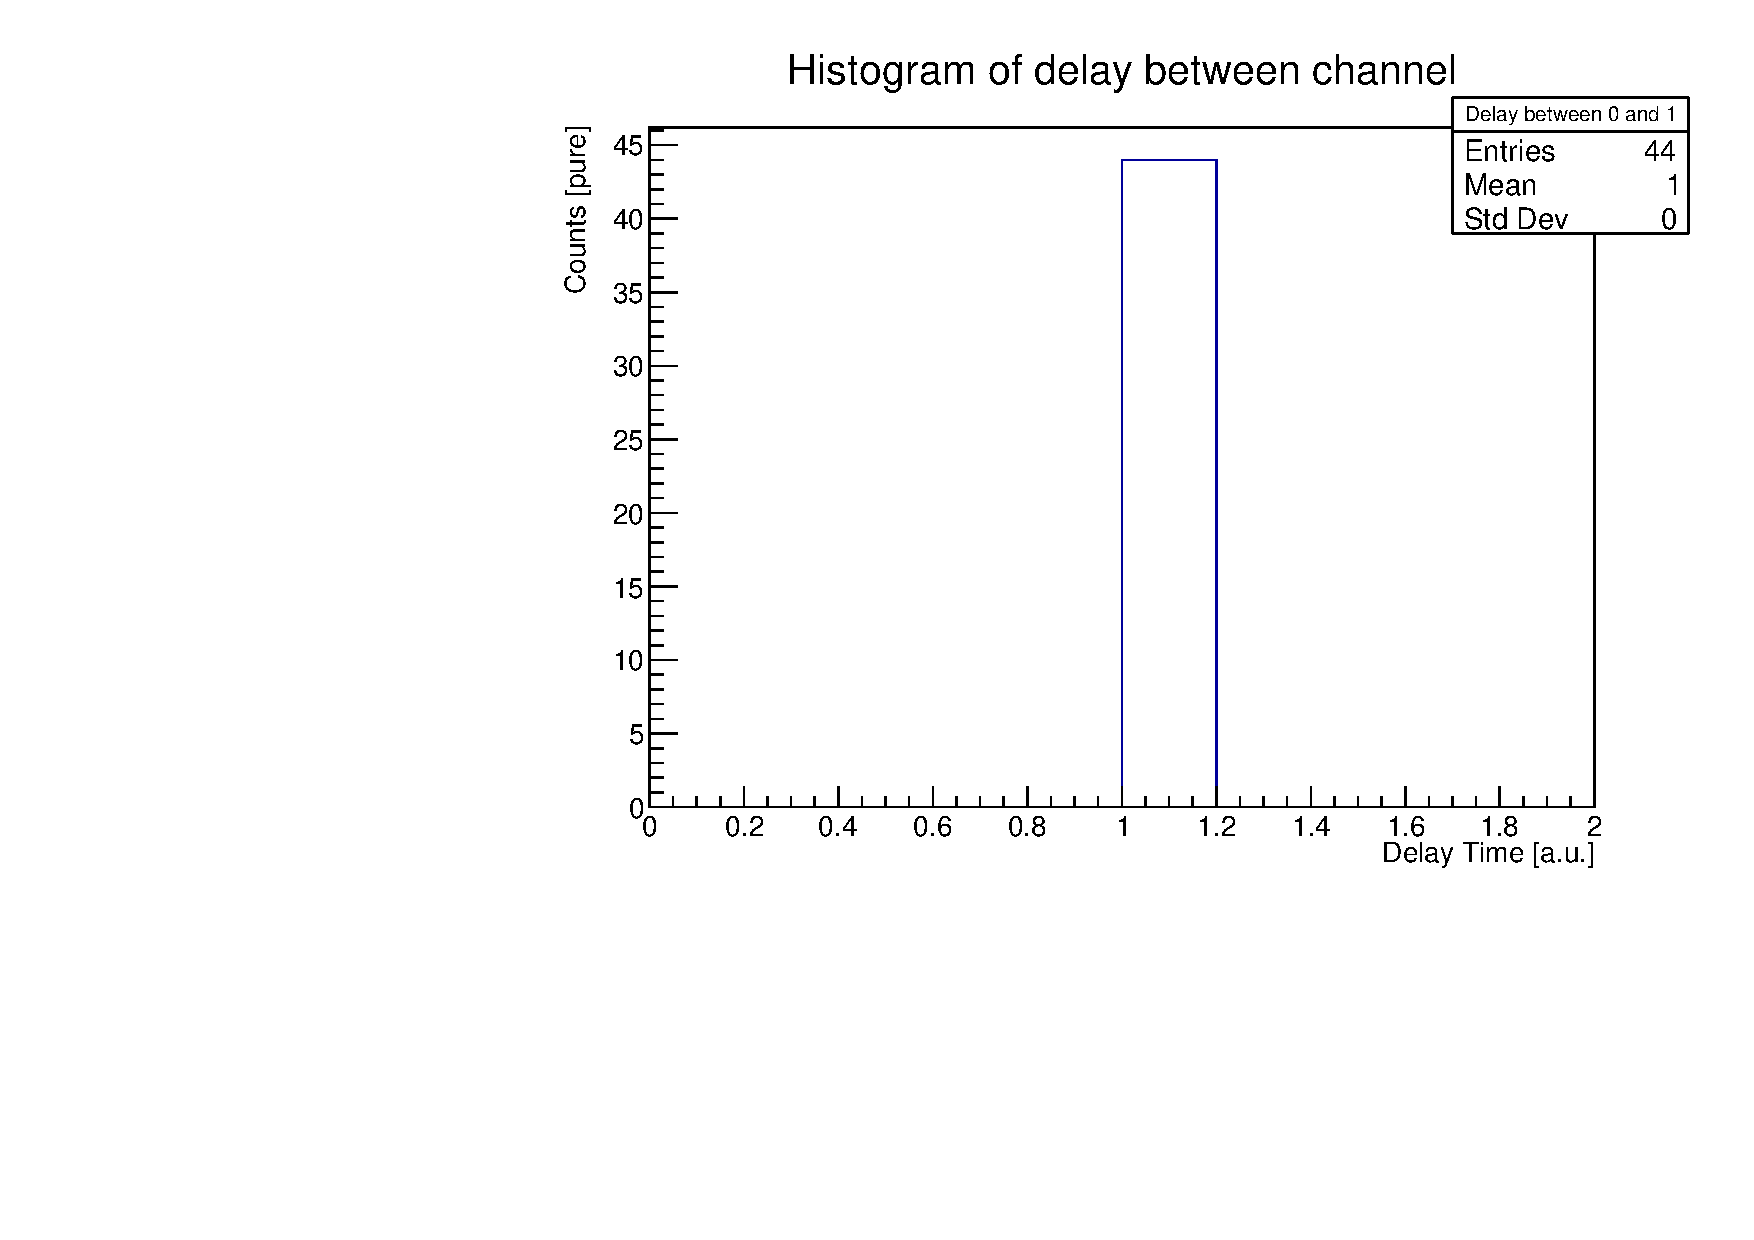
\includegraphics[width=\linewidth]{Grafici/Ritardo.pdf}
        \caption{Ritardo fra due canali utilizzando lo stesso segnale}
        \label{fig:pCHANNEL}
    \end{minipage}
\end{figure}

Quindi, chiamata $\alpha = T[s]/T[dgt]$ la costante di calibrazione digit-tempo $\bm{\alpha = 4.98892 \pm 0.00002 }$ ns/dgt. 
Il grafico \ref{fig:pCHANNEL} realizzato inviando l'onda quadra ai CH0/1 della scheda  mostra che abbiamo un digit di differenza, corrispondente al valore di $\alpha$ in tempo.
\end{flushleft}
\section{Calibrazione dell'ADC}\label{appx:calib_adc}
\begin{flushleft}

Per ottenere la costante di calibrazione che converte le unità arbitrarie in $eV$ tilizziamo il fatto che l'energia rilasciata nello scintillatore è proporzionale alla quantità di luce emessa, a sua volta proporzionale all'altezza dei segnali in uscita dal PMT.
Utilizziamo quindi come sorgente di calibrazione i raggi cosmici e supponiamo che essi siano MIP\footnote{Minimum Ionizing Particle:Una MIP (Minimum Ionizing Particle) è una particella carica che attraversa un materiale perdendo energia per ionizzazione/eccitazione con un valore di $<dE/dx>$ vicino al minimo previsto dalla curva di Bethe–Bloch} per cui la loro perdita di energia nella materia è data dalla seguente relazione:
\begin{equation}
    \label{Energy_loss}
    -\frac{1}{\rho}\frac{dE}{dx} = 2\frac{MeV \cdot cm^{2}}{g} 
\end{equation}
Possiamo considerare il materiale plastico di cui è fatto il nostro scintillatore approssimabile a carbonio la cui densità è $\rho_C \simeq 1 \frac{g}{cm^{3}}$ da cui note le dimensione di ogni lastra  (vedi sezione \ref{sec:apparato} ) è possibile ricavare l'energia rilasciata al passaggio della particella nel mezzo pari a $\Delta E  = 60MeV$. 
Per fare in modo che l'integratore campioni i segnali corretti usiamo come segnale di trigger:$(07\land04\land01)$ (coincidenza tripla), questa combinazione data la geometria dell'apparato ci assicura con ragionevole certezza che l'evento rappresenta il passaggio un raggio cosmico. 
A ciascun canale dell'integratore colleghiamo l'uscita di un PMT del blocco, che poi viene mandata a un canale dell'ADC. Calibriamo ciascun canale singolarmente, in modo da avere maggiore informazione a nostra disposizione. 
Usiamo la somma dei canali per effettuare la calibrazione, andando a rapportare il valore di energia rilasciata con il valore medio della distribuzione delle ampiezze misurato. Abbiamo optato per calibrare la derivata numerica della somma dei segnali d'output dell'integratore, al fine di semplificare l'analisi dati. 

Otteniamo così una costante di calibrazione $\bm{C=0.0564706 \frac{MeV}{dgt}}$ \\
\begin{figure}[H]
    \centering
    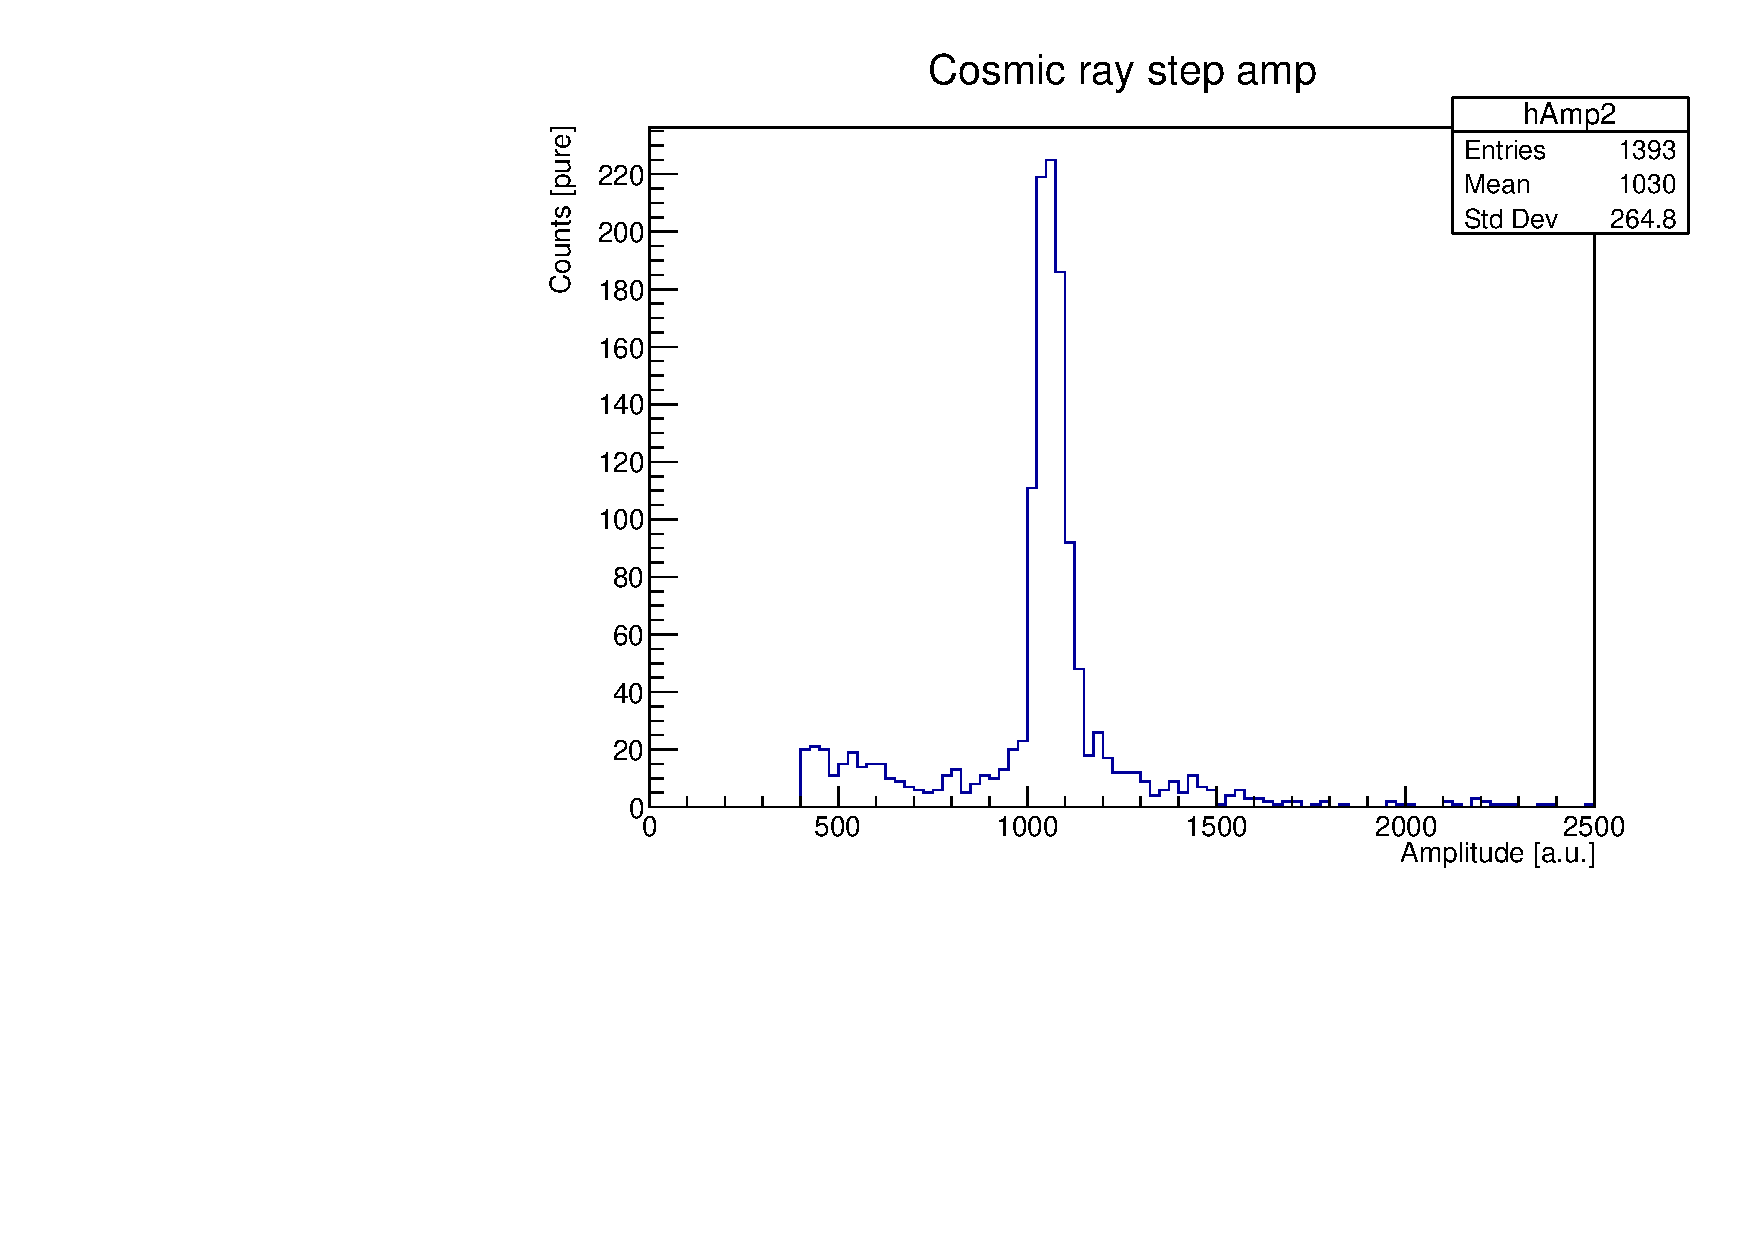
\includegraphics[width=0.5\linewidth]{Immagini/calib.pdf}
    \caption{Istogramma delle ampiezze delle utilizzato per la calibrazione.}
    \label{fig:calib_spettro}
\end{figure}

\end{flushleft}
\newpage
\section{Istogramma singoli PMT}\label{sec:plot_pmt}
\begin{flushleft}
Il codice scritto permette anche di distinguere in quale dei PMT del bersaglio è originato il segnale di STOP che accoppiato allo START definisce il tempo dt di cui realizziamo l'istogramma.\\
Al fine di avere un'analisi completa è stato realizzato il plot con relativo fit realizzato come nella sezione \ref{subsec:fit_vita_media}
Si riportano quindi i grafici ottenuti:
\begin{figure}[H]
    \centering
    \begin{minipage}{0.48\linewidth}
        \centering
        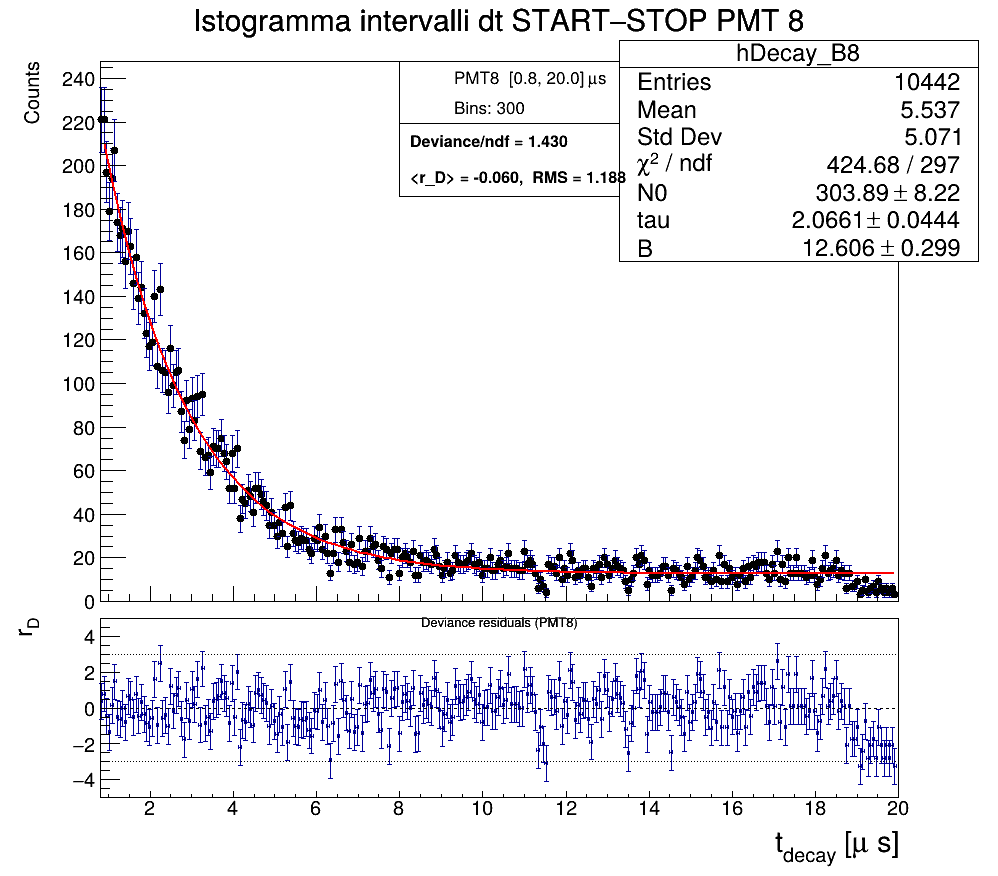
\includegraphics[width=0.8\linewidth]{Grafici_fit_finale/mu_decay_fit_PMT8_0.800_20.000_300_bins_withdevres.png}
        \caption{Risultati del fit con residui per gli eventi di PMT08}
        \label{fig:fit_pmt8}
    \end{minipage}
    \hfill
    \begin{minipage}{0.48\linewidth}
        \centering
        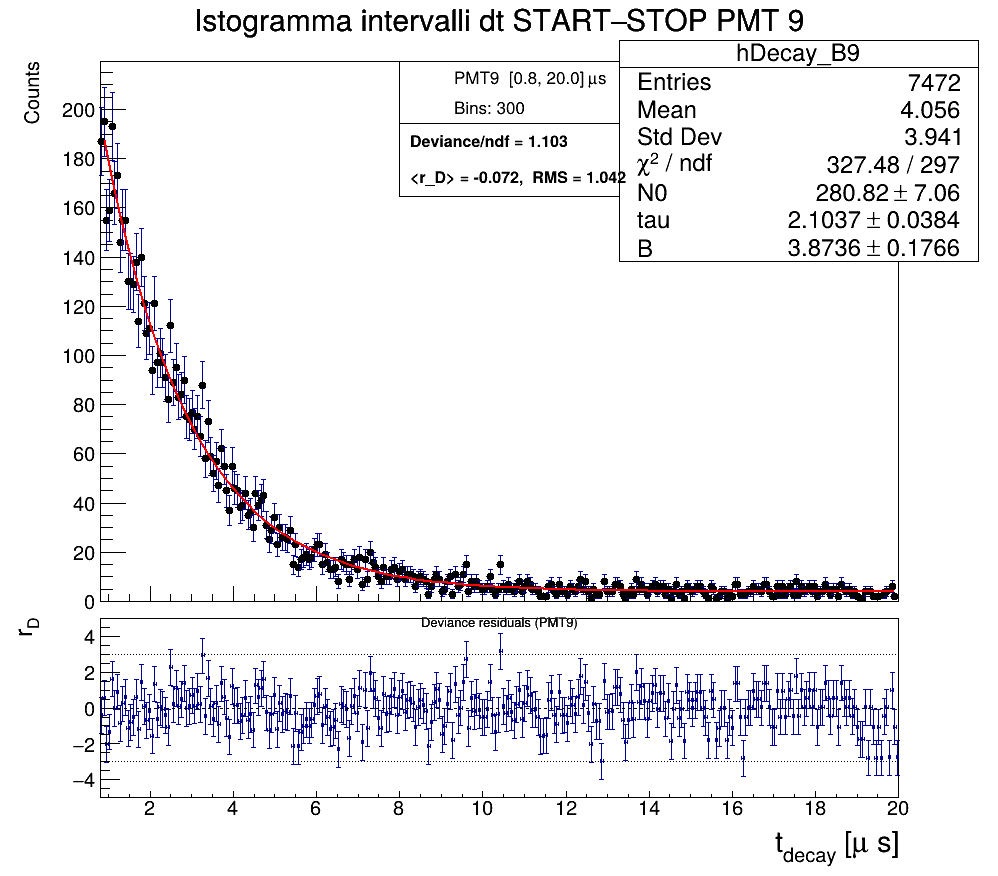
\includegraphics[width=0.8\linewidth]{Grafici_fit_finale/mu_decay_fit_PMT9_0.800_20.000_300_bins_withdevres.png}
        \caption{Risultati del fit con residui per gli eventi di PMT08}
        \label{fig:fit_pmt9}
    \end{minipage}
    \hfill
    \centering
    \begin{minipage}{0.48\linewidth}
        \centering
        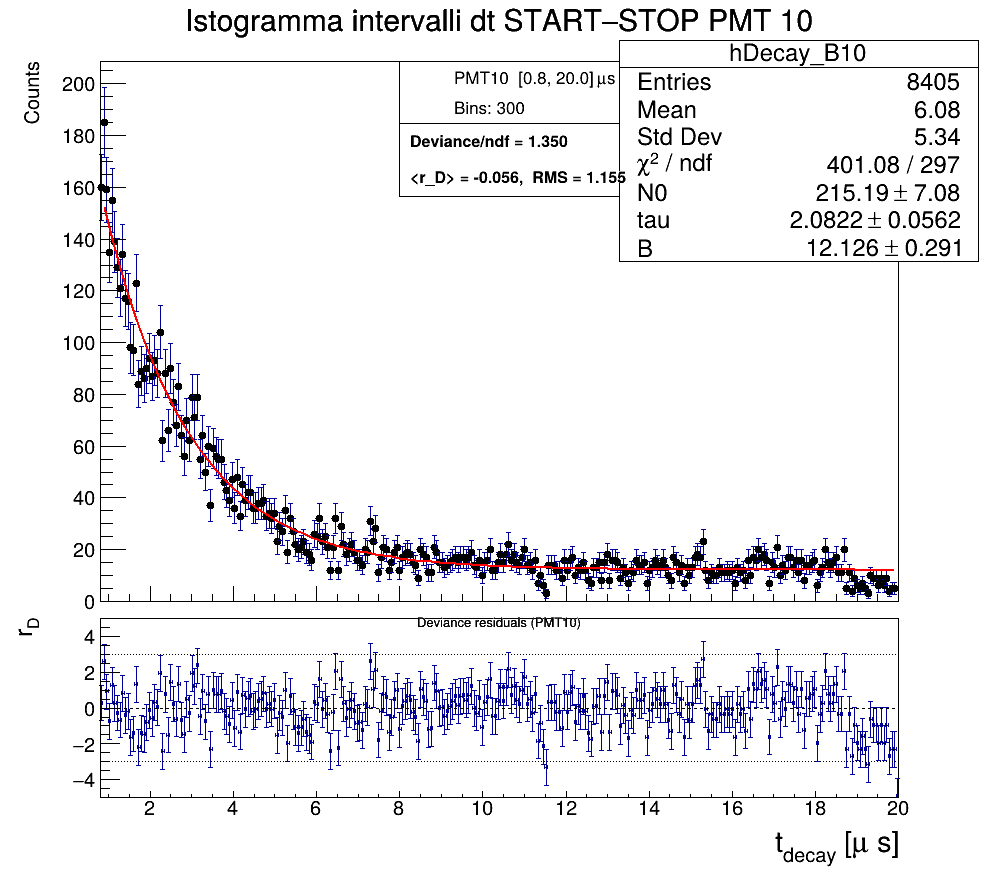
\includegraphics[width=0.8\linewidth]{Grafici_fit_finale/mu_decay_fit_PMT10_0.800_20.000_300_bins_withdevres.png}
        \caption{Risultati del fit con residui per gli eventi di PMT10}
        \label{fig:fit_pmt8}
    \end{minipage}
    \hfill
    \begin{minipage}{0.48\linewidth}
        \centering
        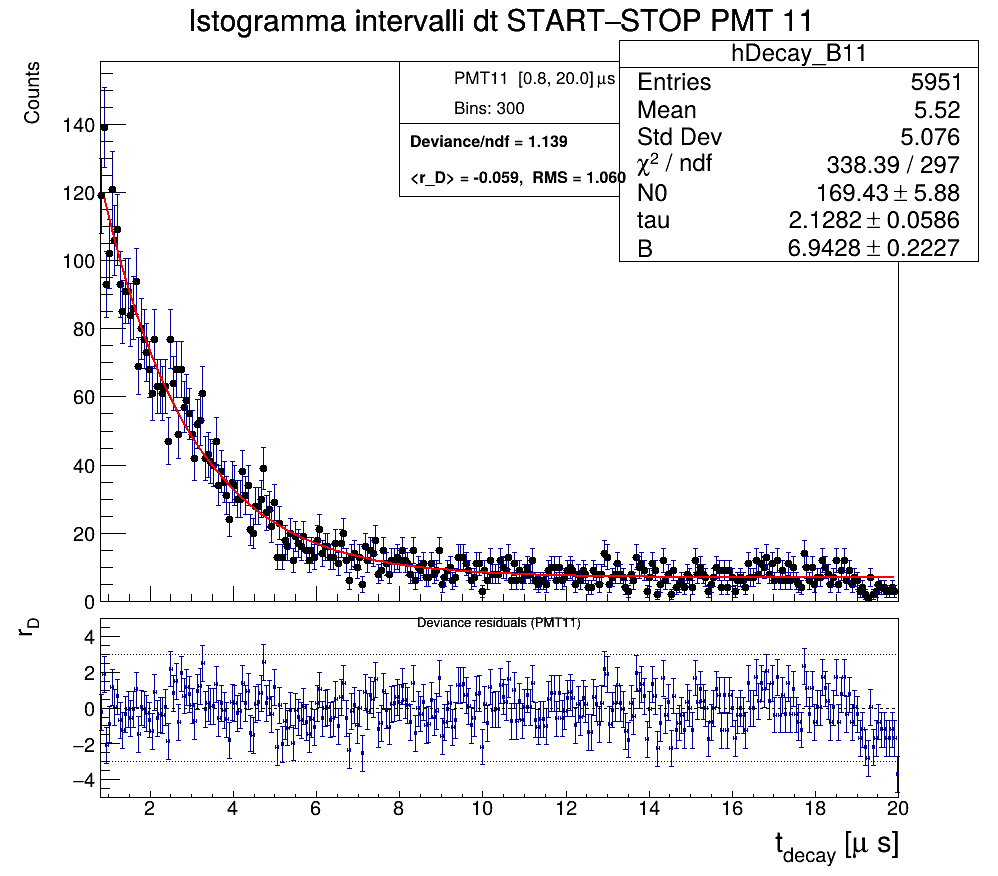
\includegraphics[width=0.8\linewidth]{Grafici_fit_finale/mu_decay_fit_PMT11_0.800_20.000_300_bins_withdevres.png}
        \caption{Risultati del fit con residui per gli eventi di PMT11}
        \label{fig:fit_pmt9}
    \end{minipage}
\end{figure}
La ricostruzione dell'andamento per ogni PMT permette di analizzare ed evidenziare nel caso criticità presenti in eventuali scintillatori o fotomoltiplicatori, nel nostro caso non si notano particolari anomalia se non un numero di conteggi inferiore rispetto agli altri PMT da parte del numero 11.\\
\end{flushleft}

\section{Grafico fit a doppio esponenziale}
\label{app:grafico_double}
\begin{figure}[H]
        \centering
        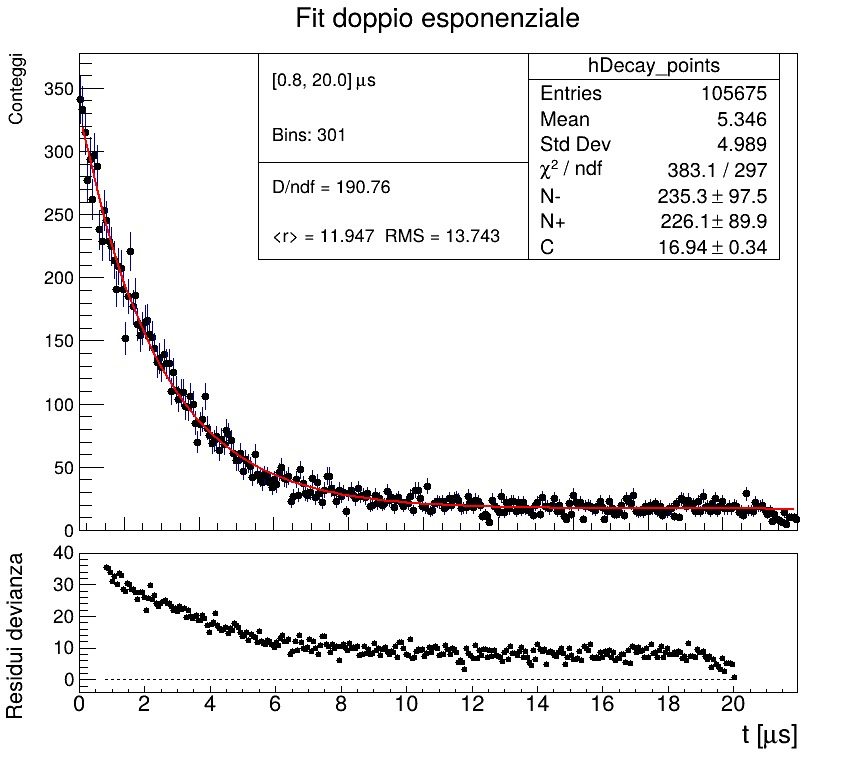
\includegraphics[width=0.8\linewidth]{Grafici/fit_double.jpeg}
        \caption{Grafico per il fit a doppio esponenziale con plot dei residui}
        \label{fig:fit_double_graph}
\end{figure}
\end{document}
